\documentclass[11pt,a4paper]{article}

\usepackage[T1]{fontenc}
\usepackage[utf8]{inputenc}
\usepackage{lmodern}
\usepackage{microtype}
\usepackage[margin=2.4cm]{geometry}
\usepackage{amsmath,amssymb}
\usepackage{graphicx}
\usepackage{booktabs}
\usepackage{tabularx}
\usepackage{threeparttable}
\usepackage{float}
\usepackage{caption}
\usepackage{enumitem}
\usepackage[table]{xcolor}
\usepackage[numbers,sort&compress]{natbib}
\usepackage[hidelinks]{hyperref}

\definecolor{spruce}{HTML}{1E3B33}
\captionsetup{font=small,labelfont=bf}
\setlist{itemsep=2pt,topsep=4pt}
\setlength{\parskip}{4pt}
\renewcommand{\arraystretch}{1.15}
\newcolumntype{Y}{>{\raggedright\arraybackslash}X}
\graphicspath{{figures/}}

\title{\textbf{Yellowstone Trophic Cascade:\\ A Time-Series Analysis}\\[6pt]
\large Wolves, elk, streamside vegetation, snow, rivers and visitors, 1911--2026,\\ with Isle Royale as a comparison system}
\author{MATH F428 Time Series Analysis and Forecasting\\
BITS Pilani, K K Birla Goa Campus\\[10pt]
\begin{tabular}{ll}
Ashwath Chandramouli & 2024ADPS0853G \\
Nitin Sureshkumar & 2024ADPS0881G \\
Tanishk Milind Tasgaonkar & 2024ADPS0874G \\
Leora Modi & 2023B4AD0866G
\end{tabular}}
\date{}

\begin{document}
\maketitle

\begin{abstract}
\noindent Gray wolves were reintroduced to Yellowstone National Park in 1995--96. The classic account holds that they set off a top-down trophic cascade: fewer elk, less browsing and recovering streamside willows. Critics argue that hunting, drought, winter severity, bison and stream hydrology explain much of the same change. We test the links of this chain with time-series methods, in four parts. Part~1 models annual growth of the northern Yellowstone elk count (1984--2025); Part~2 studies streamside vegetation from Landsat NDVI (1984--2026), snowpack, and 116 years of daily river flow; Part~3 models 564 months of park visitation (1979--2025); Part~4 applies the same methods to wolves and moose on Isle Royale (1959--2015), a system with no hunting, bison or migration. In Yellowstone, lagged wolf changes do not significantly predict elk growth (wolf-only coefficient $-0.031$ per ten wolves, $p=0.12$; VAR Granger $p=0.18$). On Isle Royale, under one shared specification, wolves clearly predict and limit moose (common-window coefficient $-23.7$ log-growth percentage points per ten wolves, $p=0.002$; Granger $p=0.009$). Streamside vegetation greened relative to nearby slopes only on Blacktail Deer Creek ($+0.026$ NDVI per decade since 1996, $p<0.001$); on the braided Lamar and Soda Butte channels, floods dominate. Year-to-year increases in elk go with a browner riverside in the same summer ($p=0.006$), but no driver Granger-causes vegetation. The river's spring pulse now arrives about 13 days earlier than in 1950 and summer low flow is falling. Park-wide visitation did not rise with wolves; it follows climate and policy. Every multivariate model was tested for Granger causality and every fitted model's residuals were checked for white noise. The evidence is consistent with parts of the cascade but cannot establish it from annual time series alone.
\end{abstract}

\tableofcontents
\newpage

%=====================================================================
\section{Introduction}
%=====================================================================

\subsection{The debate}
Wolves were absent from Yellowstone for about 70 years before 31 wolves were released in 1995--96. In the years that followed, the northern elk herd fell from about 17{,}000 to under 5{,}000 counted animals, and some streamside stands of willow and aspen grew taller. \citet{ripple2012} interpreted this as a \emph{trophic cascade}: wolves reduced elk numbers and changed where elk browse, which released riparian vegetation.

The cascade has been challenged on several fronts. Elk were also hunted heavily outside the park in the late 1990s, drought and hard winters reduced calf survival, and a growing bison herd competes for forage \citep{macnulty2016,eberhardt2007}. In some streams incised channels and low water tables prevent willow regrowth regardless of browsing \citep{marshall2013,hobbs2024}.

\subsection{Research questions}
The project splits the cascade into links that can each be examined with time-series data.
\begin{enumerate}[label=\textbf{RQ\arabic*.}]
\item Do changes in wolf numbers help explain and predict growth of the northern Yellowstone elk count, beyond climate, hunting, bison and the herd's own past? (Part~1)
\item Did streamside vegetation become greener relative to nearby slopes after 1995, does it track elk or summer water more closely, and how have snowpack and river flow changed? (Part~2)
\item Did wolves bring tourists, and is a warmer climate changing when people visit the park? (Part~3)
\item In a simpler system with no hunting, bison or migration, do the same methods detect a wolf effect on prey? (Part~4)
\item Under one shared model, how do Yellowstone and Isle Royale compare? (Synthesis)
\end{enumerate}

\subsection{Scope}
Time-series models can show whether one variable helps \emph{predict} another (Granger causality, ARIMAX), whether a series changed at a known date (intervention and break models), and how well a model forecasts out of sample. They cannot, on their own, establish causation. Most series here have 25--56 annual observations, so tests have limited power, and a non-significant result means ``no evidence'' rather than ``no effect''.

%=====================================================================
\section{Data}
%=====================================================================
Table~\ref{tab:data} lists the data used. Every processed dataset records the source of each value and flags imputed values; imputed targets are excluded when scoring forecasts.

\begin{table}[H]
\centering\small
\caption{Data sources by part.}\label{tab:data}
\begin{tabularx}{\textwidth}{@{}l l l Y@{}}
\toprule
Part & Series & Period & Source and notes \\
\midrule
1 & Northern elk count & 1984--2025 & Northern Yellowstone Cooperative Wildlife Working Group; NPS and Montana FWP; audited whole-herd counts, imputed years flagged \\
1 & Northern-range wolves & 1995--2025 & NPS Yellowstone Wolf Project annual reports (zero before 1995) \\
1 & Bison, precipitation, PDSI, harvest & 1984--2025 & NPS bison status reports; TerraClimate via Climate Engine; Montana FWP harvest \\
2 & Landsat NDVI, 6 polygons & 1984--2026 & Climate Engine, Landsat 5/7/8/9 surface reflectance, 30\,m; riverside and nearby-slope polygons on Lamar River, Soda Butte Creek and Blacktail Deer Creek \\
2 & Daily river flow & 1911--2026 & USGS gauge 06191500, Yellowstone River at Corwin Springs (42{,}359 days) \\
2 & Snow water equivalent, temperature & 1967--2026 & NRCS SNOTEL: Northeast Entrance, Canyon, Parker Peak; combined into a winter severity index and monthly mean temperature \\
3 & Recreation visits, monthly & 1979--2025 & NPS IRMA visitor-use statistics (564 months) \\
3 & Vehicles by entrance & 1993--2026 & NPS IRMA traffic counts \\
4 & Wolf and moose counts & 1959--2019 & Wolves and Moose of Isle Royale project (R package \texttt{dsem}) \\
4 & Wolf and moose counts & 1980--2026 & NPS, extends the series past 2019; robustness check \\
4 & Winter climate & 1959--2011 & NE Minnesota climate division (R package \texttt{MARSS}) \\
\bottomrule
\end{tabularx}
\end{table}

Three data issues shape the analysis. First, elk survey methods and survey areas changed over time; Part~1 audits each value and treats 2020--21 whole-herd coverage as unresolved. Second, NPS switched from manual visitor counts to traffic-counter estimates in 1993, two years before the wolf release, so Part~3 controls for it. Third, the Isle Royale project series is a revised reconstruction that is smoother than raw aerial counts; Part~4 re-runs key models on the NPS series.

%=====================================================================
\section{Methods}
%=====================================================================
All parts follow the Box--Jenkins cycle of identification, estimation and diagnostic checking \citep{box2015}, with shared conventions.

\paragraph{Transformations and stationarity.} Counts are modelled on the log scale and, where needed, as annual log growth $r_t=\log N_t-\log N_{t-1}$. Stationarity is assessed with the augmented Dickey--Fuller test (null: unit root) together with KPSS (null: stationarity); a series is treated as stationary only when the two agree. Seasonal series are decomposed with STL. Monotonic trends use Mann--Kendall tests with Sen's slope, with the Hamed--Rao correction for autocorrelation.

\paragraph{Univariate and transfer-function models.} ARMA and SARIMA orders are identified from the ACF and PACF and compared by AIC and BIC. Exogenous drivers enter as ARIMAX regressions, and known events (wolf release, floods, counting changes) as intervention terms. Where residual autocorrelation is likely, standard errors are Newey--West or the errors are modelled explicitly as AR(1).

\paragraph{Granger causality.} For a $k$-variable VAR($p$),
\begin{equation}
\mathbf{y}_t=\mathbf{c}+\sum_{i=1}^{p}A_i\,\mathbf{y}_{t-i}+\mathbf{u}_t ,
\end{equation}
$x$ does not Granger-cause $y$ if every coefficient on lagged $x$ in the $y$ equation is zero \citep{granger1969}. This is tested with an $F$ test, in both directions. The VAR is fitted to stationary series, with lag chosen by information criteria. Part~4 also uses the Toda--Yamamoto levels test, which remains valid when the order of integration is uncertain. A Granger test is only valid if the VAR's residuals are white noise, so this is checked each time. \emph{Instantaneous causality} tests whether the two equations' shocks are correlated in the same period.

\paragraph{Residual diagnostics.} Every fitted model's residuals are tested for remaining autocorrelation with the Ljung--Box statistic \citep{ljungbox1978},
\begin{equation}
Q(h)=n(n+2)\sum_{k=1}^{h}\frac{\hat\rho_k^2}{n-k}\ \sim\ \chi^2_{h-m},
\end{equation}
where $m$ is the number of ARMA parameters, and for VARs with its multivariate form (the Portmanteau test). Constant variance is checked with Engle's ARCH LM test \citep{engle1982}. A model whose residuals are not white noise is revised (more lags, AR errors or a different order) before its results are used.

\paragraph{Volatility, breaks and extremes.} Changing volatility is modelled with GARCH(1,1) and EGARCH(1,1). Structural breaks are located by exact dynamic programming with BIC choosing the number of breaks. Return periods of extreme floods use GEV and Gumbel fits.

\paragraph{Mechanistic models.} Part~4 fits Lotka--Volterra and Rosenzweig--MacArthur predator--prey equations and a stochastic population simulation. Part~2 fits a degree-day snowmelt equation \citep{hock2003}. Part~1 fits a state-space model separating process from observation error.

\paragraph{Forecast evaluation.} Models are compared out of sample by rolling-origin forecasts: refit on data up to each origin, forecast ahead, score with MAE, MAPE or MASE, and compare against naive benchmarks (no change, drift, seasonal naive, climatology). Differences are tested with Diebold--Mariano where the sample allows.

%=====================================================================
\section{Part 1: Yellowstone elk and wolves}
%=====================================================================
\subsection{Model}
The outcome is the annual log growth of the northern elk count, $y_t=\log E_t-\log E_{t-1}$. ADF and KPSS agree that $y_t$ is stationary and its ARMA identification selects white noise, so the drivers model is an ARIMAX(0,1,0) on log elk:
\begin{equation}
y_t=\mu+\beta_W\,\frac{W_{t-1}-W_{t-2}}{10}+\boldsymbol{\gamma}'\mathbf{x}_t+\varepsilon_t ,
\end{equation}
where $W$ is the northern-range wolf count and $\mathbf{x}_t$ contains bison, NDVI, precipitation, PDSI, harvest rate and winter severity. Each variable's predictive role is tested alone and in a full model. Figure~\ref{fig:p1series} shows the series.

\begin{figure}[H]
\centering
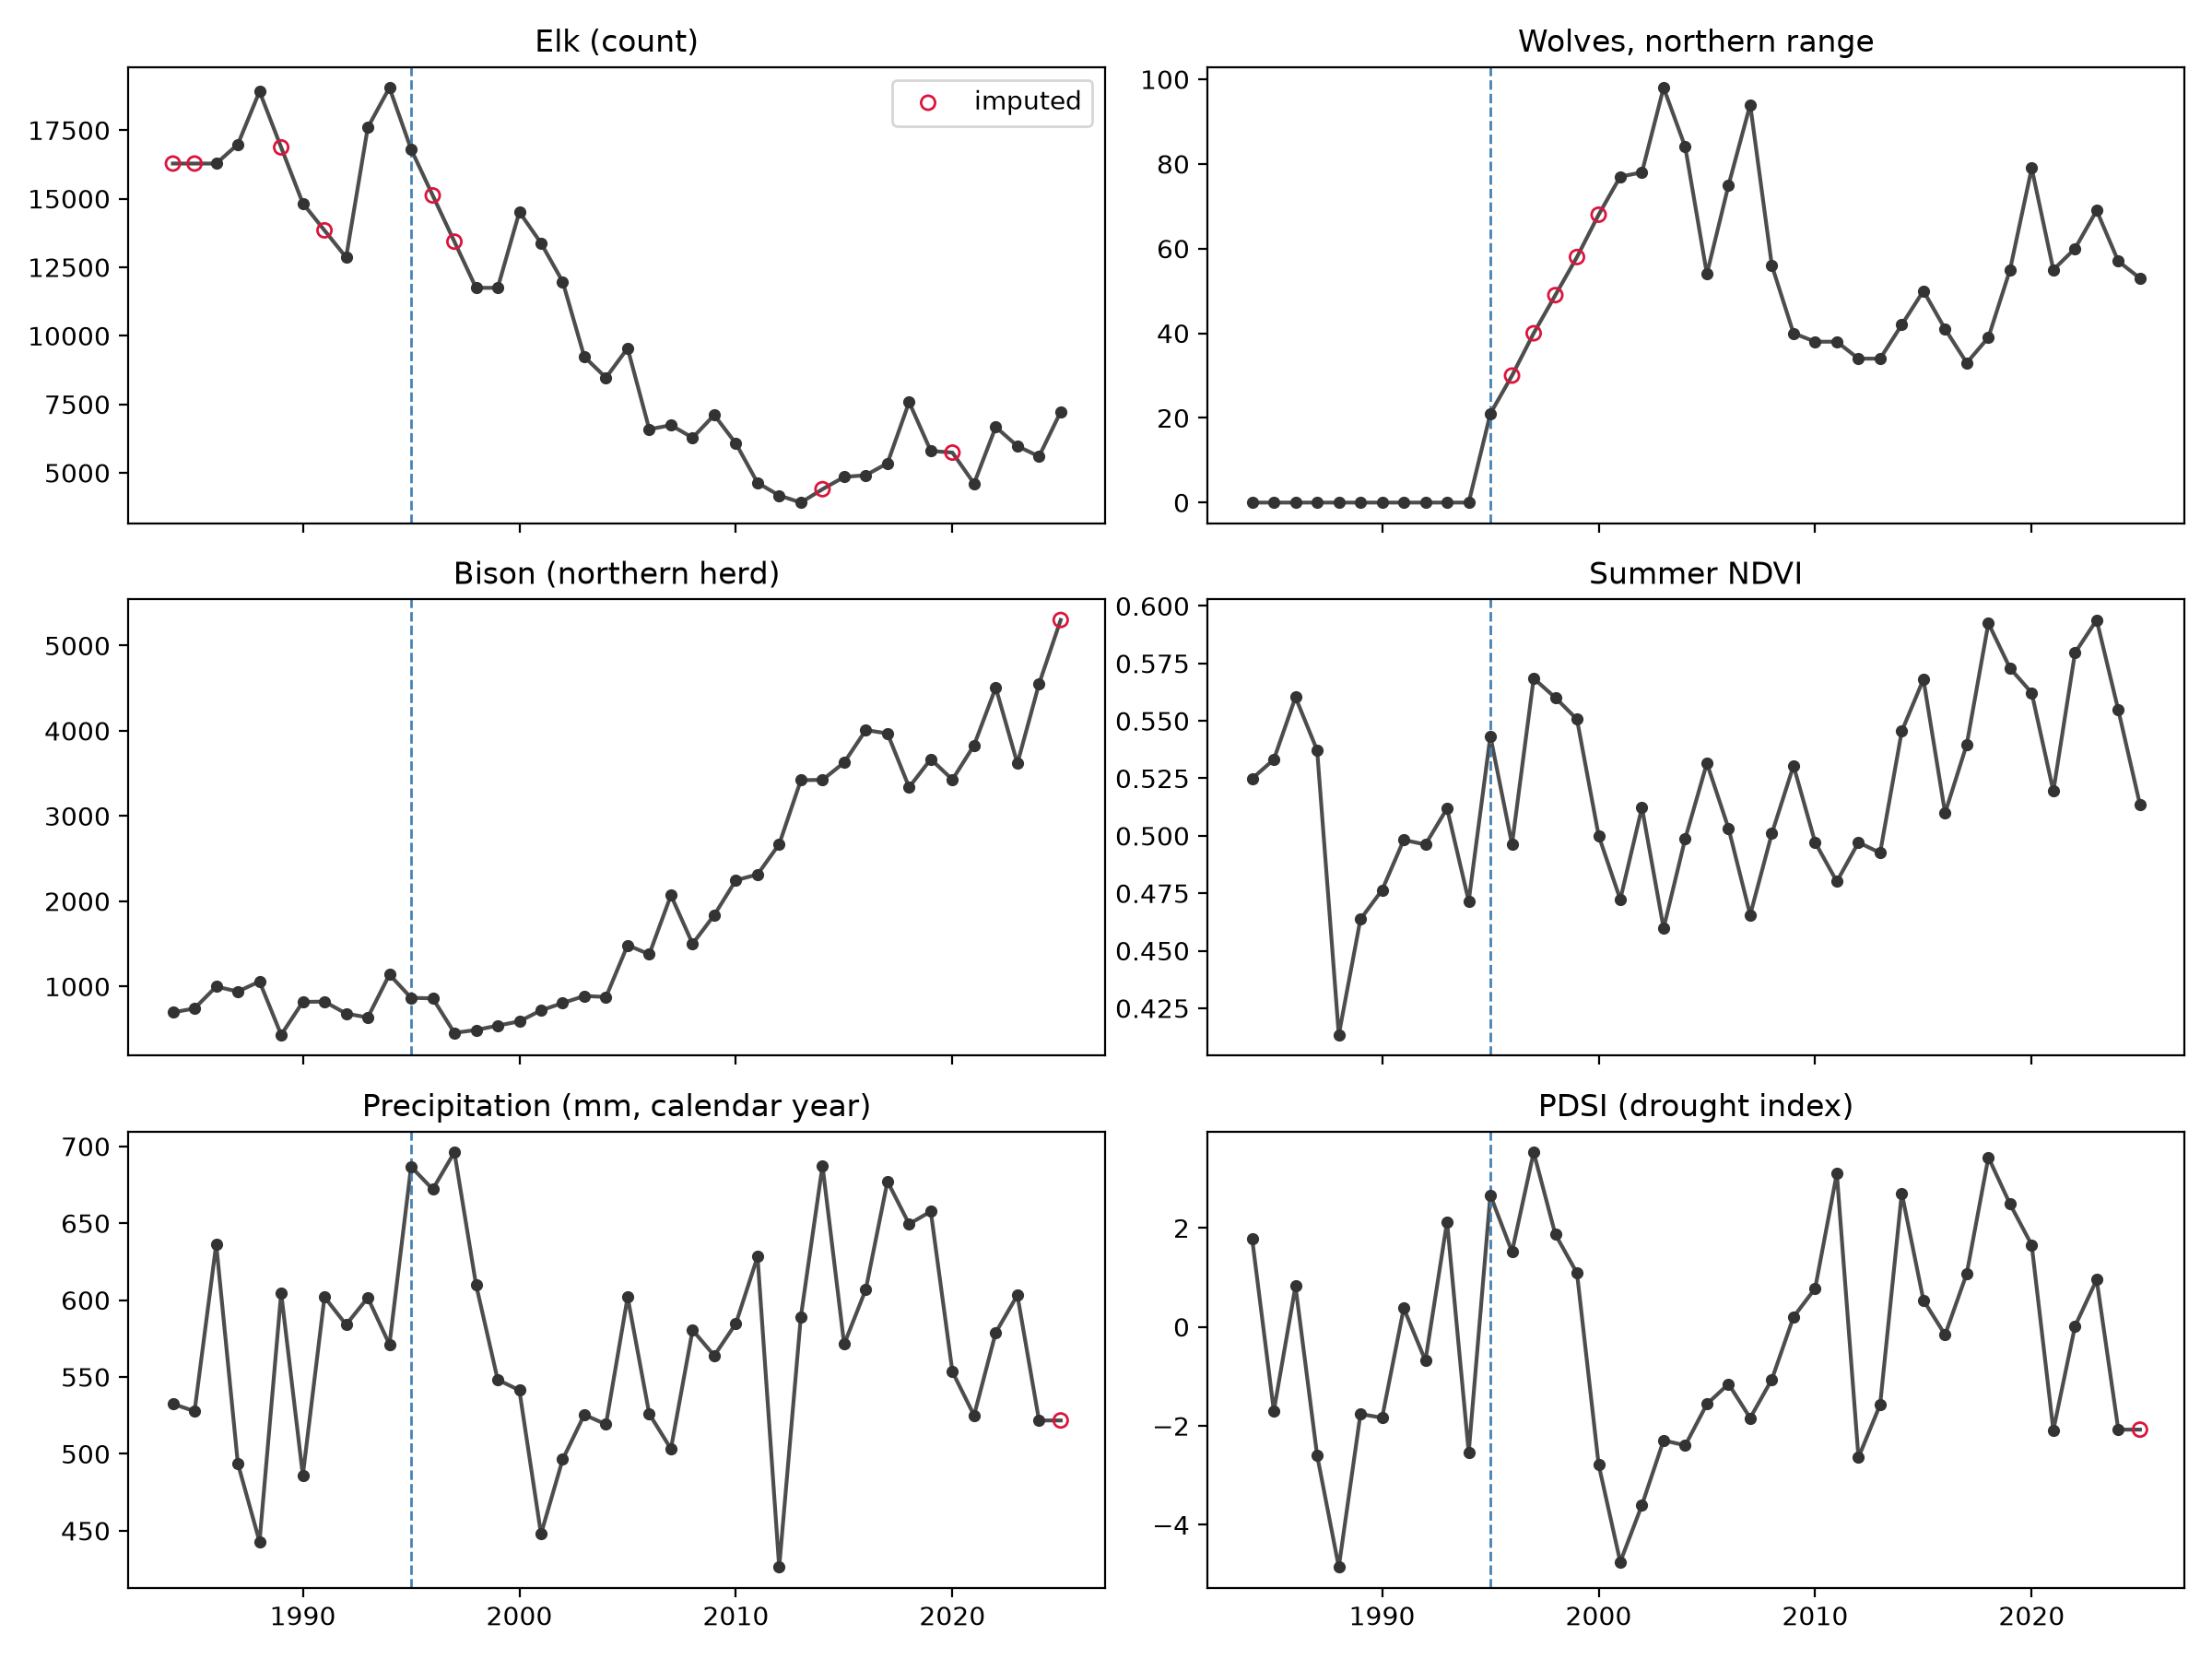
\includegraphics[width=0.82\textwidth]{p1_all_series.png}
\caption{Part 1 series, 1984--2025. Open circles are imputed values; the dashed line marks 1995.}\label{fig:p1series}
\end{figure}

\subsection{Results}
\begin{itemize}
\item \textbf{Drivers (Q1).} The wolf-only coefficient is $-0.0305$ log growth per ten-wolf increase (95\% CI $-0.069$ to $+0.008$; $p=0.120$; $n=40$). In the full model it is $-0.0273$ ($p=0.408$). The interval includes both a substantial negative and a small positive association, so the data cannot distinguish them.
\item \textbf{Feedback and Granger causality (Q2).} In the prespecified VAR(1) on elk growth and wolf changes (1997--2025), wolves do not Granger-cause elk ($p=0.176$) and elk do not Granger-cause wolves ($p=0.797$); at lag~2, $p=0.136$ and $0.182$. AIC and BIC both prefer zero lags.
\item \textbf{Forecasting (Q3).} Over nine common eligible years, the wolf-only model's MAE is 986.4 elk against 1{,}003.8 for drift, a 1.7\% gain; the full model is worse (1{,}402.1). Replacing five interpolated wolf counts with recovered published counts barely changes this (983.1).
\item \textbf{Winter (Q4) and breaks (Q5).} The wolf $\times$ winter interaction is null ($p=0.990$). BIC selects no break in mean growth; a separate trend-break search has its minimum at 2014, which does not identify a cause.
\item \textbf{Removals (Q6).} \citet{eberhardt2007} report 12{,}512 estimated wolf kills and 11{,}653 hunting removals over 1996--2004. Wolf kills exceed the published hunt from 2000 onward. In a joint standardised regression neither wolves ($p=0.145$) nor harvest ($p=0.907$) is significant, so counts alone cannot rank the two.
\item \textbf{Viability (Q7) and observation error (R).} From 27 observed transitions, drift is $-0.0157$ and volatility $0.179$; the Gompertz coefficient $\phi=0.997$ is close to a random walk (bootstrap LR $p=0.986$). The illustrative probability of the count crossing below 4{,}000 within ten years is 38.7\% (bootstrap 6.9--78.7\%). A state-space model gives process SD 0.112 and observation SD 0.087.
\end{itemize}

\subsection{Residual checks}
All ARIMAX residuals pass Ljung--Box at lags 5 and 8 ($p=0.64$--$0.97$) and the ARCH test ($p\ge0.11$). For this report we also checked the VAR used for the Granger tests: its residuals pass the multivariate Portmanteau test (8 lags, $p=0.54$ for VAR(1), $0.85$ for VAR(2)), so the Granger $p$-values above are valid.

\subsection{Answer to RQ1}
The annual series gives limited evidence that wolf changes alone explain or predict elk growth. This does not show that wolves have no effect: the sample is short, survey methods changed, and wolves overlap in time with heavy hunting and drought.

%=====================================================================
\section{Part 2: Vegetation, snow and river}
%=====================================================================
\subsection{Design}
The cascade claim is about streamside willows, so Part~2 measures greenness where the claim is made. For three northern-range streams, Landsat NDVI is extracted for a \emph{riverside} polygon and a nearby \emph{slope} polygon. The annual statistic is the median, over all July--August images, of the riverside$-$slope difference on the same image date. Weather, drought, haze and sensor changes affect both polygons alike and largely cancel; what remains is specific to the riverside. Climate Engine exports leave partial rows without placeholders, so only complete rows are used (599 of 1{,}003 and 590 of 692 image dates). The water side of the debate uses daily flow of the Yellowstone River since 1911 and three SNOTEL stations, summarised by water year (October--September).

\subsection{Did the riverside green up after 1995?}
\begin{figure}[H]
\centering
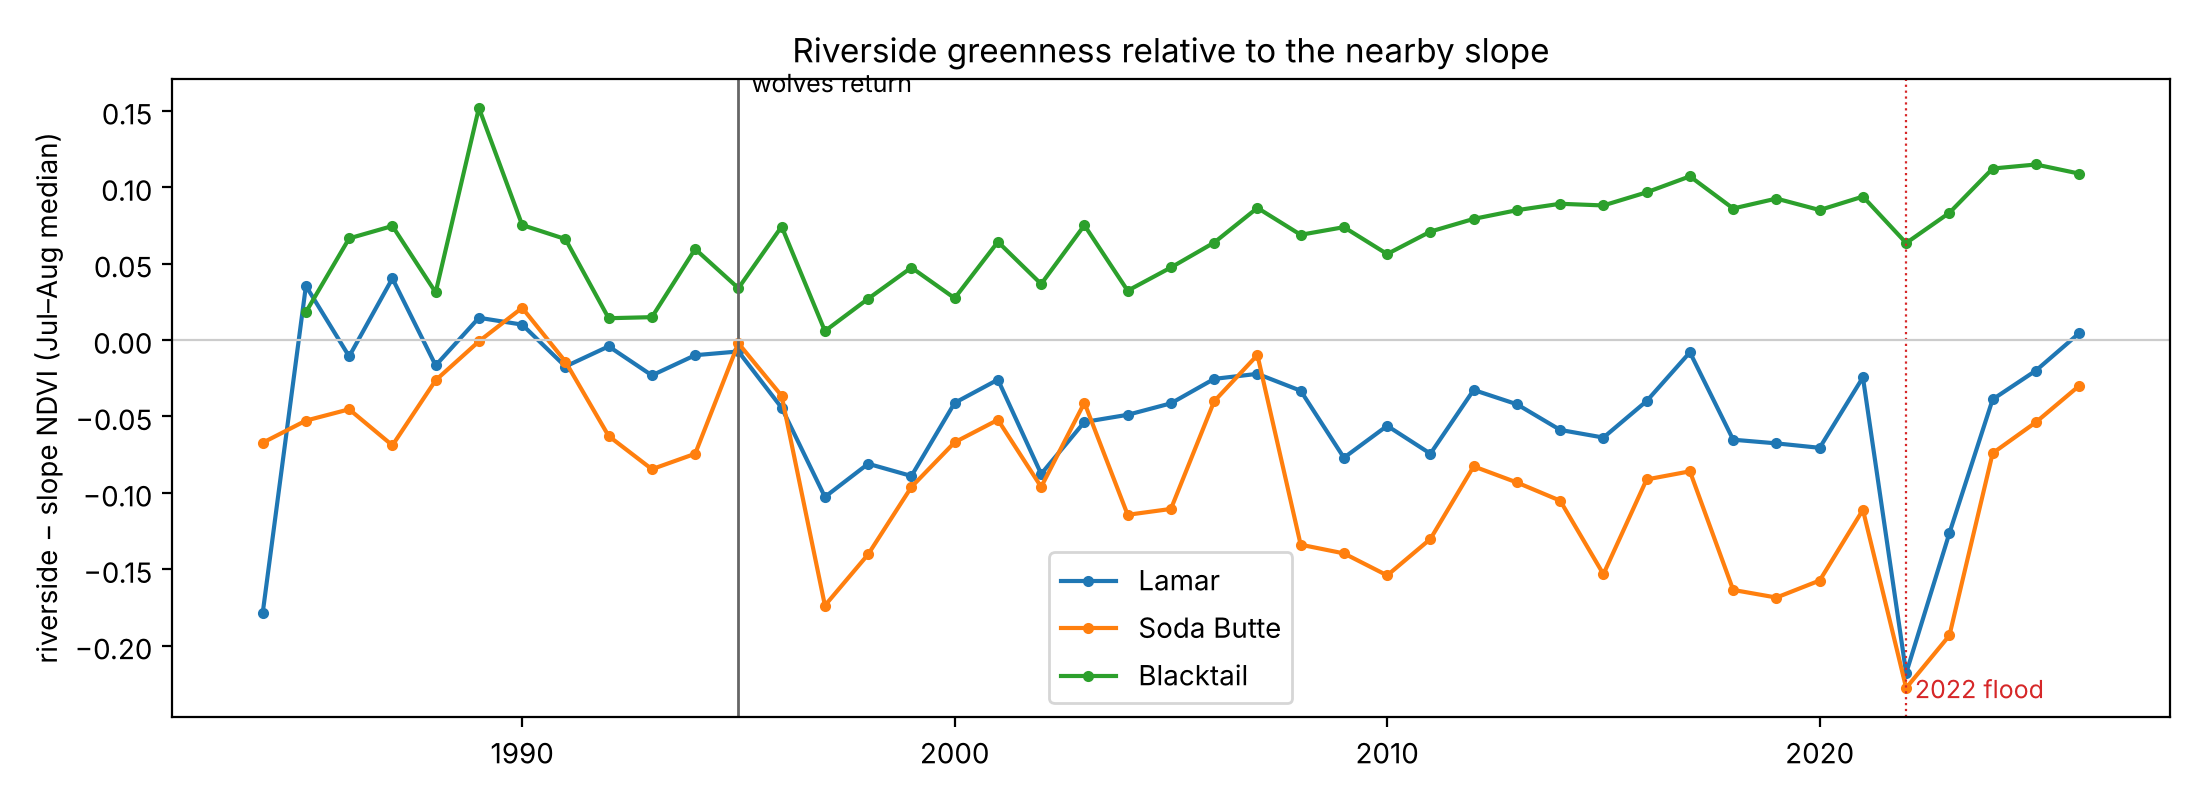
\includegraphics[width=\textwidth]{P2_10_riverside_minus_slope.png}
\caption{Riverside minus slope NDVI, July--August median, 1984--2026.}\label{fig:veg}
\end{figure}

The answer depends on the stream (Figure~\ref{fig:veg}).
\begin{itemize}
\item \textbf{Blacktail Deer Creek}, a narrow willow-lined creek and the one \citet{ripple2012} studied, greened relative to its slope after 1995: Sen's slope $+0.026$ NDVI per decade over 1996--2026 (Mann--Kendall $p<0.001$), with a break chosen by BIC in 2007 and no trend before 1995. The rise is already present within the Landsat 5/7 era (1996--2012, $p=0.02$), so it is not an artefact of the 2013 sensor change. It is gradual, not a step at 1995, as expected if willows slowly escape browsing.
\item \textbf{Lamar River and Soda Butte Creek}, wide braided gravel channels, show no greening: both differences fall over 1984--2026 ($p=0.018$ and $0.009$). Soda Butte's break is at 1997, and both drop sharply that year, after the third and fourth largest river peaks in 116 years (1997 and 1996) and in the same way as after the record 2022 flood. The wolf release and two major floods occurred within two years of each other, a real confound for any before/after-1995 comparison.
\end{itemize}
In the intervention regression $d_y=a+bt+c\,\mathrm{post}_{1995}+e\,(t-1995)\,\mathrm{post}_{1995}$, Lamar's step at 1995 is $-0.066$ with Newey--West errors ($p=0.03$) but not significant once the errors are modelled as AR(1) ($p=0.28$); Blacktail's post-1995 change in trend becomes significant with AR(1) errors ($+0.004$ per year, $p=0.04$). Pooled over the three streams there is no 1995 effect.

\subsection{Water or elk?}
\citet{marshall2013} argued that low water tables, not only browsing, hold willows back. The riverside difference was regressed on standardised summer 7-day low flow, log elk and log bison, pooled with a separate intercept per stream. Because elk and bison trend, the same model was fitted in first differences.

\begin{table}[H]
\centering\small
\caption{Riverside$-$slope difference on year-to-year changes in drivers, three streams pooled ($n=122$). Coefficients per standard deviation; errors clustered by year.}\label{tab:fd}
\begin{tabular}{@{}lccc@{}}
\toprule
Change in & Coefficient & 95\% CI & $p$ \\
\midrule
Summer 7-day low flow & $-0.0097$ & $[-0.018,\,-0.002]$ & 0.020 \\
Log elk count & $-0.0447$ & $[-0.077,\,-0.013]$ & 0.006 \\
Log bison count & $+0.0035$ & $[-0.045,\,+0.052]$ & 0.888 \\
\bottomrule
\end{tabular}
\end{table}

Years when elk increase go with a browner riverside relative to slope that summer, which is consistent with browsing (Table~\ref{tab:fd}). Wetter late summers go with a \emph{smaller} difference in every specification. The likely reason is the design: in wet summers the slopes green up strongly while the always-wet riverside changes less, so this metric cannot isolate water-table limitation.

\paragraph{Granger causality.} Each series was first made stationary (Lamar's difference and low flow are stationary in levels by ADF and KPSS; Soda Butte, Blacktail, log elk and log bison are differenced). In pairwise tests at lags 1 and 2 for each stream, no driver Granger-causes the riverside difference: all 18 tests have $p\ge0.20$. A four-variable VAR(1) for each stream gives the same result ($p=0.20$--$0.89$), and the reverse-direction sanity checks are also null. The elk and water links are within the same year, not lagged.

\paragraph{Residual checks.} The VARs' residuals pass the Portmanteau test (8 lags, $p=0.48$--$0.76$). Single-stream regressions and the first-difference model pass Ljung--Box (lags 5 and 10) and ARCH; the Soda Butte intervention model failed Ljung--Box at lag~5 ($p=0.03$) and passes once refitted with AR(1) errors ($\phi=0.39$). Pooled models in levels leave stream-specific drift in their residuals for Blacktail and Soda Butte, which is why the first-difference and single-stream results are the ones reported.

\subsection{Has snowmelt shifted?}
\begin{figure}[H]
\centering
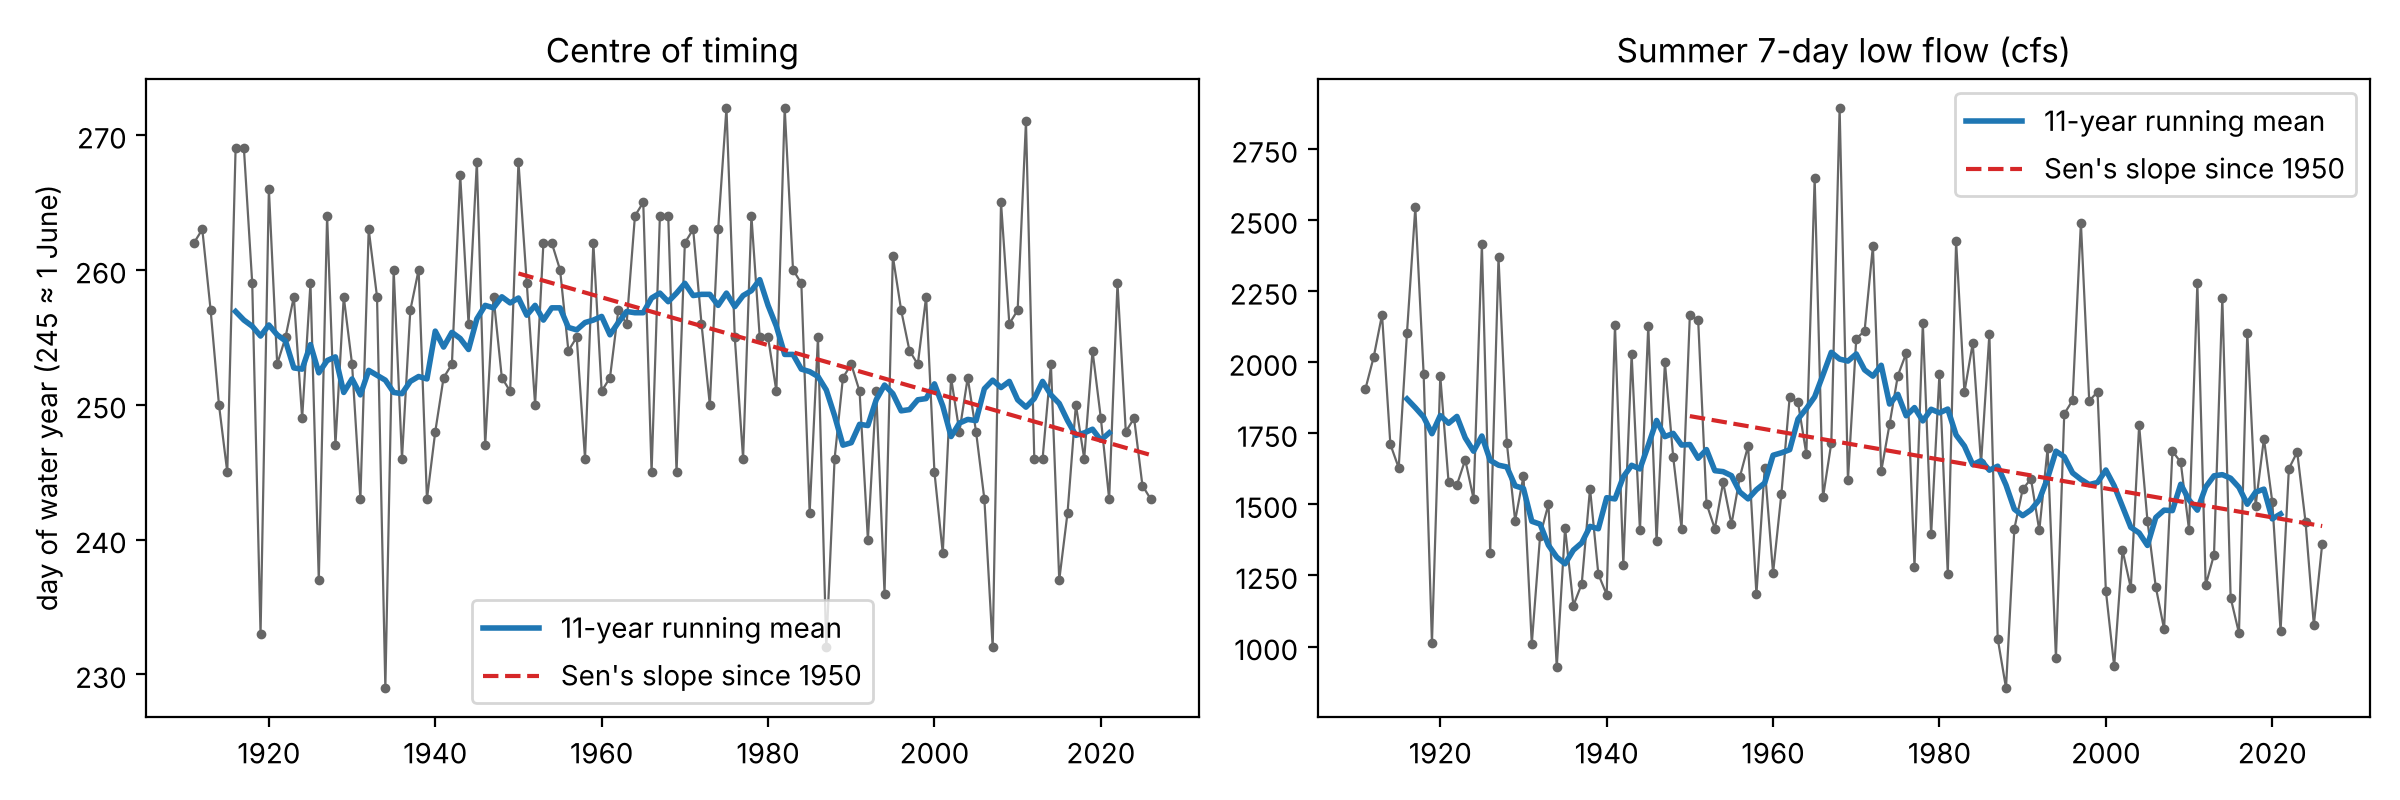
\includegraphics[width=\textwidth]{P2_03_timing_lowflow.png}
\caption{Centre of timing of annual flow (left) and summer 7-day low flow (right), water years 1911--2026.}\label{fig:timing}
\end{figure}

The centre of timing (CT), the day by which half of a water year's flow has passed, has moved earlier by 0.8 days per decade since 1911 ($p=0.002$) and 1.8 days per decade since 1950 ($p=0.0001$ after the autocorrelation correction), about 13 days in total (Figure~\ref{fig:timing}). The annual peak has moved earlier at a similar rate ($-1.9$ days per decade since 1950, $p=0.002$) and the April--May share of annual flow is rising ($p<0.001$). Annual mean flow has no trend, but summer 7-day low flow has fallen by about 3\% per decade since 1950 ($p=0.026$): the water arrives earlier, and late summer is drier. Peak snow water equivalent at Northeast Entrance has fallen by 0.9 inches per decade since 1967 ($p=0.005$), while the three-station severity index shows no trend since 1982.

\subsection{Does snow set the river? A degree-day melt model}
Later snow melt-out moves the river's centre of timing later by 0.67 days per day ($R^2=0.78$), and a larger snowpack raises annual flow (log mean flow $+0.21$ per SD of peak SWE, $R^2=0.68$). The residuals of these regressions pass Ljung--Box and ARCH.

The simplest physical model of snowmelt says snow melts in proportion to how far the air is above freezing:
\begin{equation}
\frac{d\,\mathrm{SWE}}{dt}=-k\,\max(T-T_0,\,0),\qquad T_0=0^\circ\mathrm{C}.
\end{equation}
For each year at Northeast Entrance, the model is started at that year's peak snowpack and stepped forward one day at a time with that year's temperatures and $k$ equal to the median of the \emph{other} years (leave-one-out). The median melt factor is 3.1\,mm per $^\circ$C-day, within the 2--7 range reported for seasonal snow \citep{hock2003}. The model predicts melt-out with a mean absolute error of 4.1 days (bias $-0.8$ days, $r=0.93$), against 9.6 days for always predicting the average day (Figure~\ref{fig:dd}). Its yearly errors are white noise (Ljung--Box $p=0.68$ and $0.27$ at lags 5 and 10).

\begin{figure}[H]
\centering
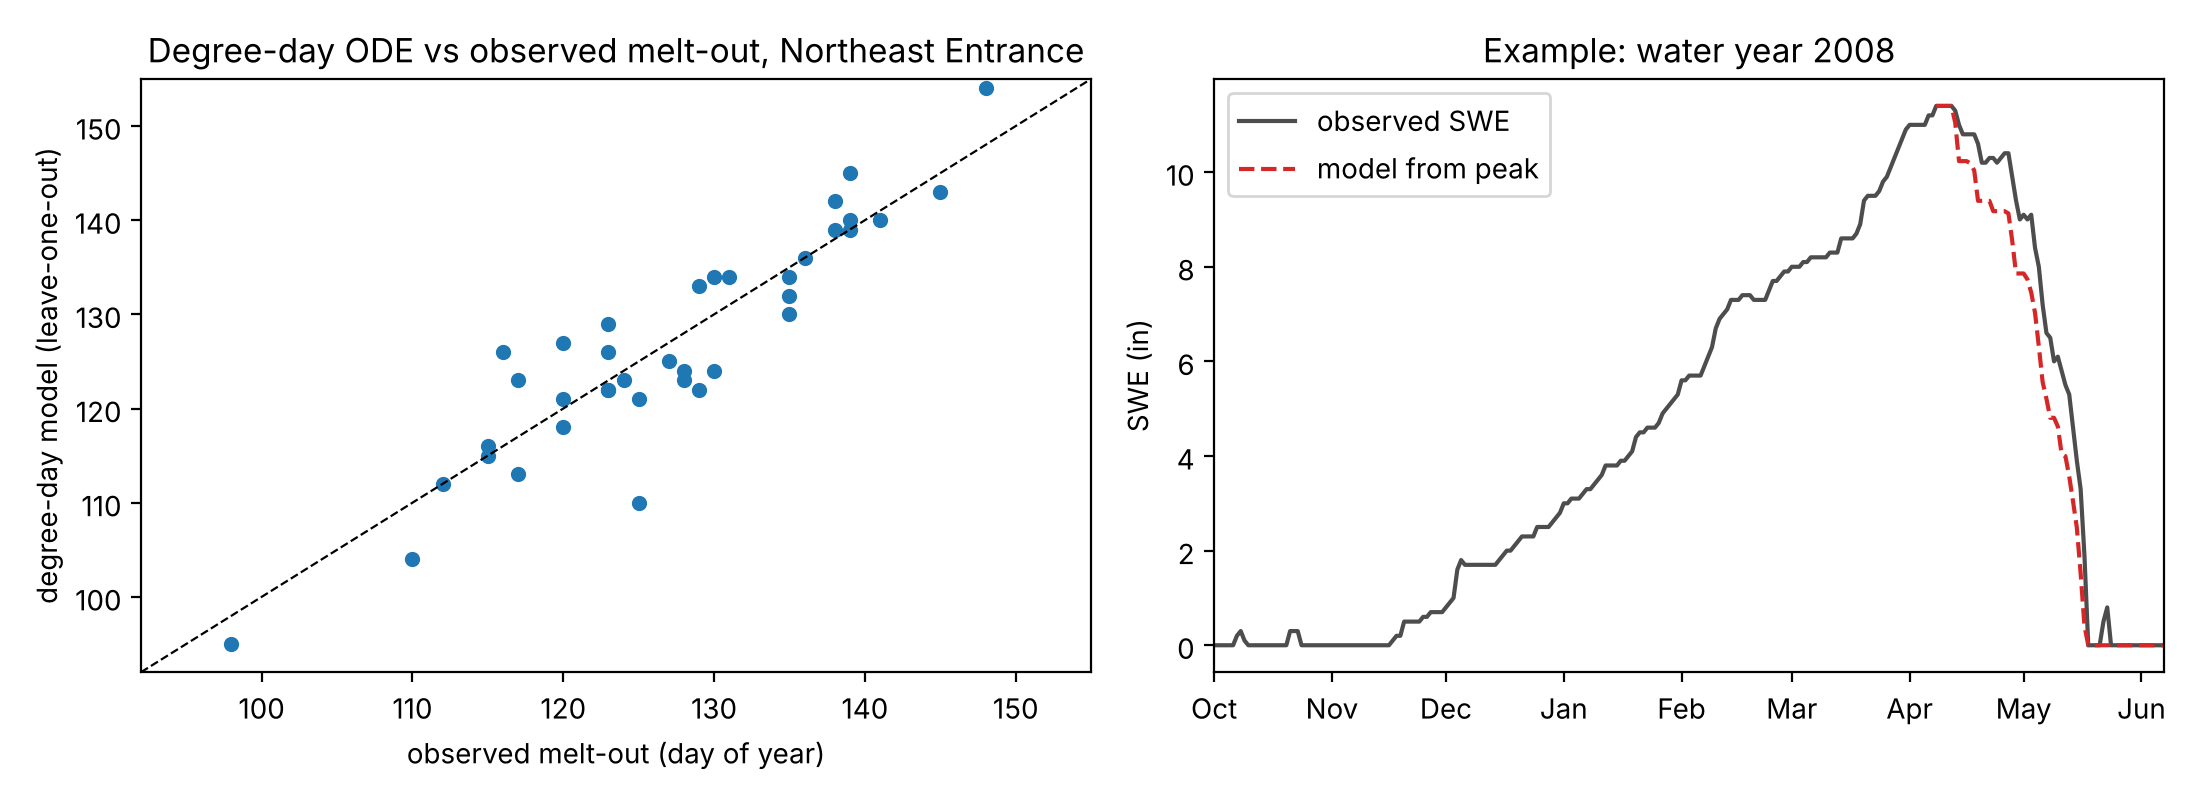
\includegraphics[width=0.95\textwidth]{P2_05_degree_day.png}
\caption{Degree-day model: leave-one-out predicted against observed melt-out (left) and an example year (right).}\label{fig:dd}
\end{figure}

\paragraph{Granger causality.} VARs pairing snow (peak SWE, severity index, melt-out anomaly) with river features (mean flow, low flow, centre of timing), 1982--2025, test whether last winter's snow helps predict this year's river. It does not: snow$\rightarrow$river $p=0.19$--$0.64$, river$\rightarrow$snow $p=0.23$--$1.00$. The same-year link is very strong (instantaneous causality $p<0.001$ for every pair). Lag length was chosen by BIC and increased where the residuals were not white; the two low-flow systems needed a second lag, after which all Portmanteau tests pass ($p=0.14$--$0.49$). There is therefore no detectable year-to-year carry-over storage at this gauge.

\subsection{Forecasting monthly flow}
Log monthly flow (1{,}392 months) needs a seasonal difference to be stationary. Candidate SARIMA models were compared by BIC, but a model was only eligible if its residuals passed Ljung--Box at lags 12, 24 and 36.

\begin{table}[H]
\centering\small
\caption{SARIMA identification for log monthly flow. Ljung--Box degrees of freedom are reduced by the number of ARMA parameters.}\label{tab:sarima}
\begin{tabular}{@{}lccccc@{}}
\toprule
Model & BIC & LB $p$ (12) & LB $p$ (24) & LB $p$ (36) & White? \\
\midrule
(1,0,2)(0,1,1)$_{12}$ & $-444.3$ & 0.23 & 0.27 & 0.04 & no \\
(3,0,0)(0,1,1)$_{12}$ & $-443.5$ & 0.20 & 0.28 & 0.04 & no \\
(1,0,0)(0,1,1)$_{12}$ & $-443.2$ & 0.01 & 0.03 & 0.01 & no \\
\textbf{(2,0,2)(0,1,1)$_{12}$} & $\mathbf{-440.2}$ & \textbf{0.42} & \textbf{0.45} & \textbf{0.08} & \textbf{yes} \\
(0,1,1)(0,1,1)$_{12}$ airline & $-258.2$ & 0.00 & 0.00 & 0.00 & no \\
\bottomrule
\end{tabular}
\end{table}

The chosen model, (2,0,2)(0,1,1)$_{12}$, leaves no residual autocorrelation above 0.08 (Figure~\ref{fig:sarres}). The three models with slightly lower BIC fail, including the (1,0,0)(0,1,1)$_{12}$ model chosen in an earlier version of the analysis. The residuals are heteroscedastic (ARCH $p<0.001$) and heavy-tailed, because snowmelt months are far more variable than winter months. This does not bias point forecasts, but SARIMA's constant-width intervals are too narrow in spring. In rolling-origin tests over water years 2017--2026 (refit each September, forecast 12 months), SARIMA's mean absolute percentage error is 20.7\%, against 22.0\% for monthly climatology and 30.2\% for seasonal naive.

\begin{figure}[H]
\centering
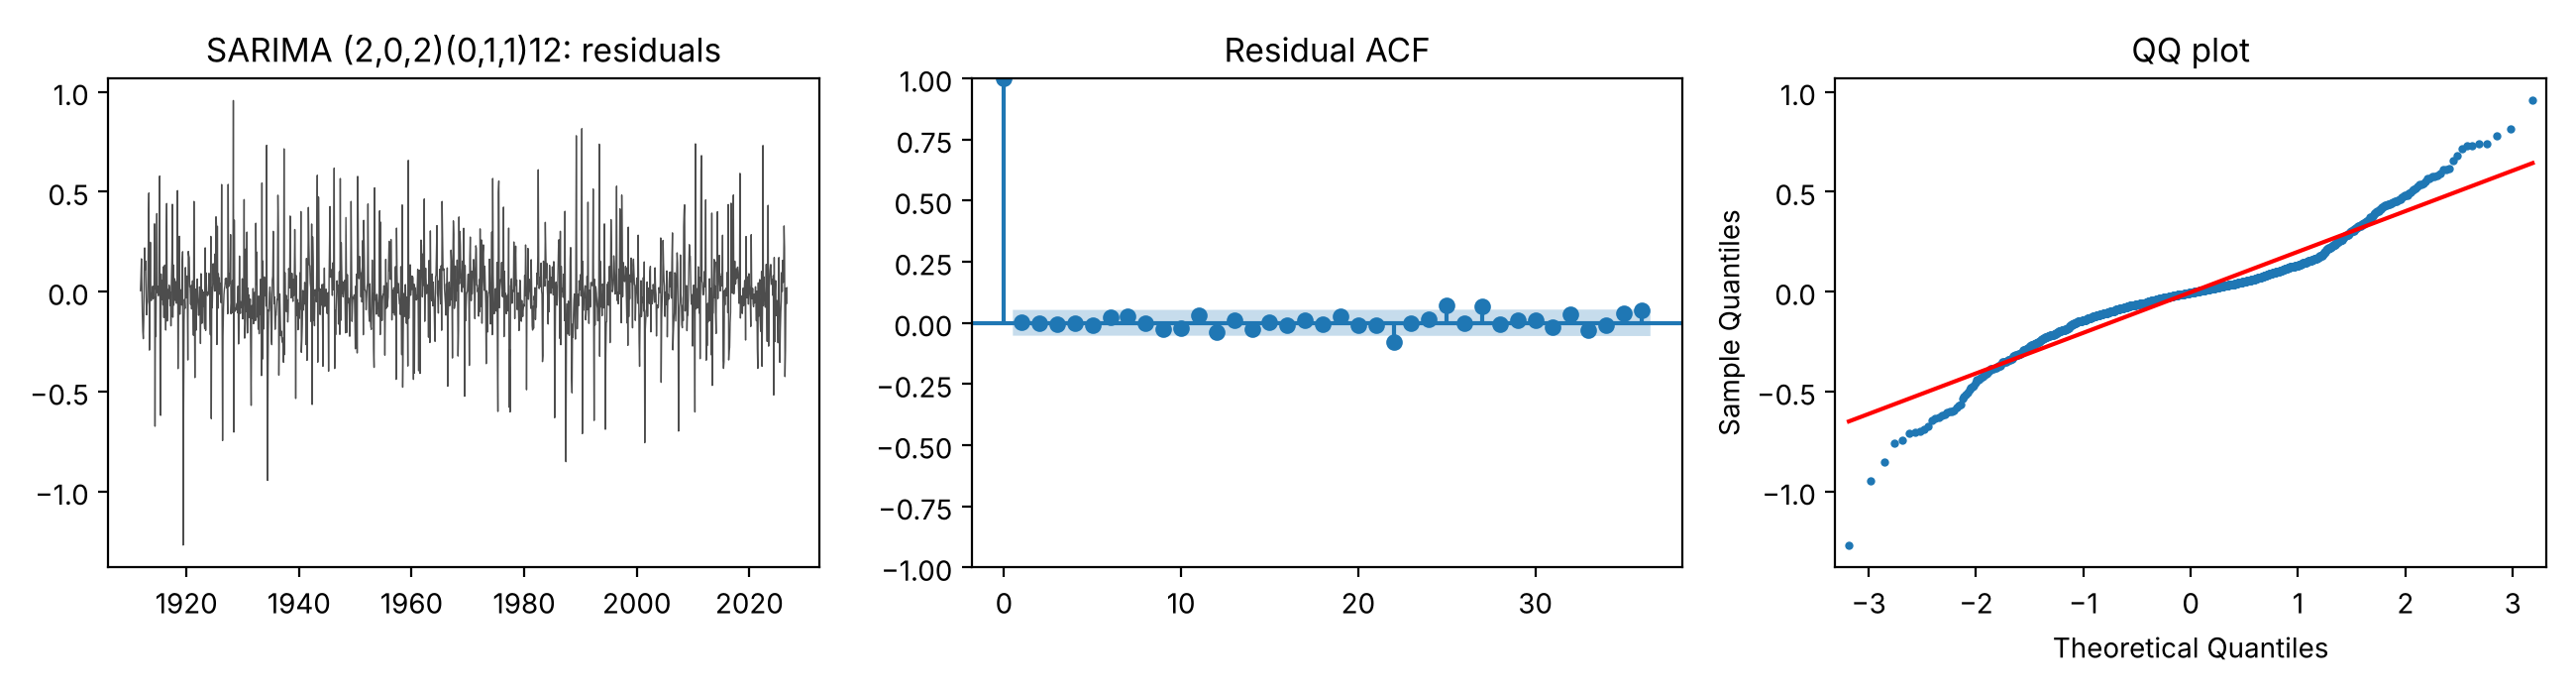
\includegraphics[width=\textwidth]{P2_13_sarima_residuals.png}
\caption{Residuals of the chosen SARIMA: time plot, ACF and normal QQ plot.}\label{fig:sarres}
\end{figure}

\subsection{Volatility and the 2022 flood}
Daily flow is converted to an anomaly $z_t$ by removing the smoothed day-of-year mean and standard deviation of log flow. As an Ornstein--Uhlenbeck process, $dz=-\theta z\,dt+\sigma\,dW$, the daily AR(1) coefficient is 0.978, so an anomaly has a half-life of 32 days. Daily shocks are 3.6 times larger in some seasons than others, so the AR residuals are scaled by their seasonal size before comparing constant-variance, GARCH(1,1) and EGARCH(1,1) models with Student-$t$ errors. EGARCH is best by BIC (100{,}538 against 107{,}661 for constant variance), with a significant asymmetry term ($\gamma=0.071$). Before any volatility model the squared shocks are autocorrelated (largest ACF 0.25); after GARCH or EGARCH this falls to 0.02, so the clustering is captured. Ljung--Box still rejects with 42{,}000 days, but at autocorrelations of 0.02 the residuals are white noise for practical purposes.

On 13 June 2022 the river peaked at 47{,}200 cubic feet per second, 48\% above the previous record of 32{,}000 (1918) and 3.7 standard deviations above normal for the date. Its return period depends almost entirely on the assumed tail: a Gumbel fit to the 1911--2021 annual peaks gives about 2{,}100 years (90\% bootstrap interval 1{,}020--5{,}458), while a GEV fit estimates a bounded tail (shape 0.118, upper limit 51{,}968 cfs) and calls the event nearly impossible. The flood collapsed the riverside$-$slope difference by 5.9 SD on Lamar and 2.5 SD on Soda Butte relative to 2017--2021, recovering over 2023--2026.

\subsection{Answer to RQ2}
Satellite evidence supports riparian recovery on the small willow-lined creek where the cascade was first reported, but not on the large braided rivers, where floods and channel form dominate. More elk go with a browner riverside in the same summer, but no driver has a lagged (Granger) effect. Snowmelt and the river now peak earlier and summer low flow is falling; each year's snow sets that year's river, with no carry-over. Caveats: 30\,m pixels mix willows with gravel, grass and water; there are only 11 pre-wolf years; the polygons are drawn on present-day imagery while channels move; and the gauge is a basin-wide water index, not the water table under these willows.

%=====================================================================
\section{Part 3: Park visitation}
%=====================================================================
\subsection{Base model}
Recreation visits rose from about 2.0 million a year (1980) to 4.8 million (2024--25), and July is about 66 times November. Log visits have a unit root; the seasonal difference is stationary. Ranked by BIC among models whose residuals pass Ljung--Box at lag 24, the base model is SARIMA(0,1,2)(1,1,1)$_{12}$ with dummies for the 1988 fires ($-35\%$), the COVID closure ($-65\%$), the 2022 flood ($-35\%$) and government shutdowns ($-36\%$). Its smallest MA root is 1.015, a sign of over-differencing, so a SARIMA(1,0,2)(1,1,1)$_{12}$ with drift (+1.6\% a year) was also fitted and compared out of sample. Residuals pass Ljung--Box at lags 12--36 but are heavy-tailed (kurtosis 14.8), so $p$-values are approximate.

\subsection{Did wolves bring tourists?}
In winter the only road open to cars runs through Lamar Valley, where wolves are watched, so winter visits were modelled as an intervention series with summer as a control (Figure~\ref{fig:p3wolves}). Every estimate of the post-1995 change in winter visits is negative and none is significant ($-15\%$ to $-22\%$, $p\ge0.43$). The monthly SARIMA, the most precise test, rules out a park-wide winter increase above about 1.5\%. Winter visits are driven by snowmobile rules ($-30\%$ after 2004). The exception is the North gate, the road to Lamar Valley: winter cars there doubled from 16.7 thousand (winter 1996) to 33.8 thousand (winter 1997) and move with the wolf count (elasticity $\approx0.3$, $p=0.02$--$0.27$ across models). A placebo regression also comes out significant, so this is suggestive, not proven.

\begin{figure}[H]
\centering
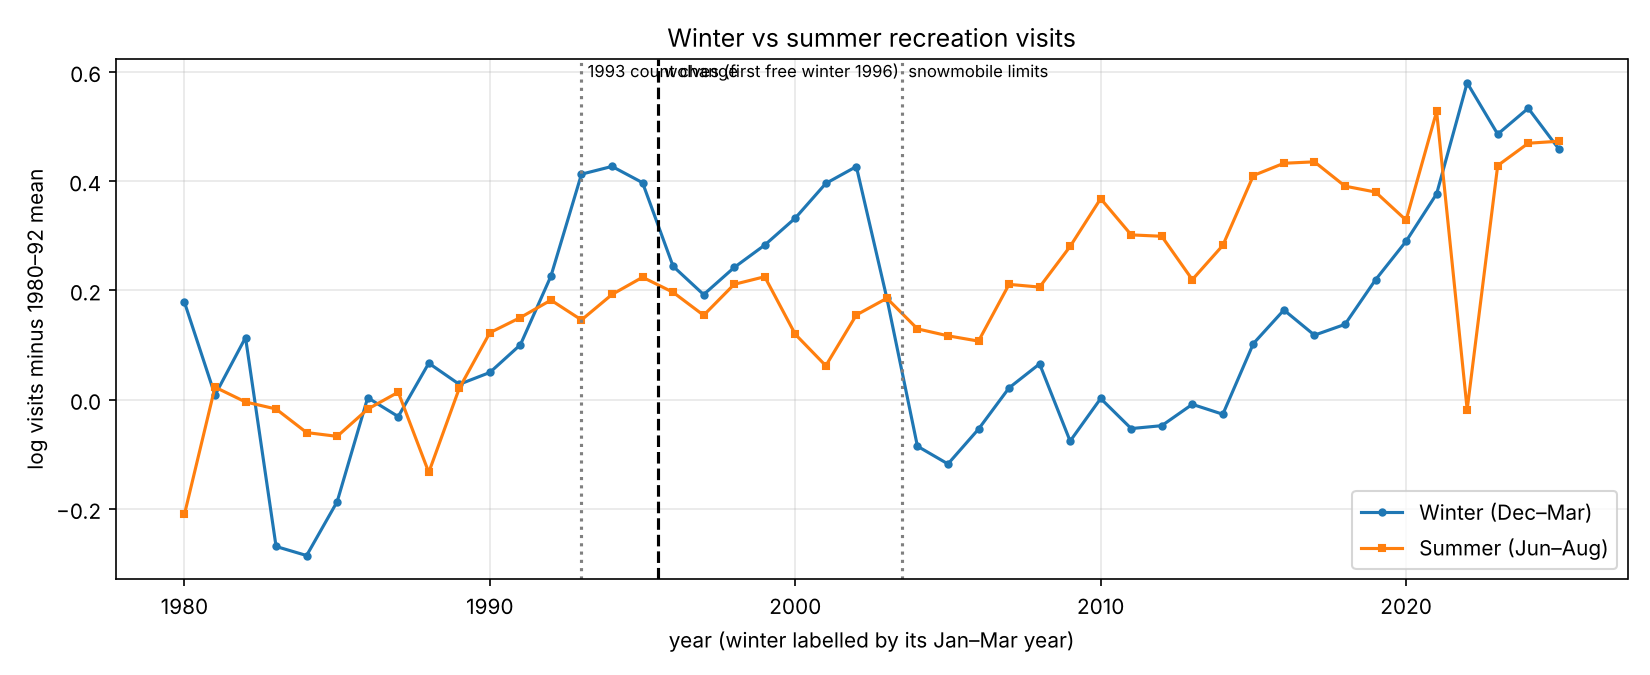
\includegraphics[width=0.8\textwidth]{q1_winter_vs_summer_1995.png}
\caption{Winter and summer visits relative to their 1980--92 mean. The jump is in 1993, when NPS changed how it counts, not in 1995.}\label{fig:p3wolves}
\end{figure}

\subsection{Is climate shifting the season?}
The share of visits in April, May, September and October rose from 24\% (1979--83) to 38\% (2021--25) (+2.6 percentage points per decade, $p<0.001$), while the visit-weighted mean month did not move ($p=0.56$): the season is stretching at both ends (Figure~\ref{fig:p3climate}). A month 1\,$^\circ$C warmer brings about 3\% more visits, and 5--9\% more in shoulder months.

\paragraph{Granger causality.} A VAR on year-on-year visit growth and year-on-year temperature change (1985--2019) tests whether past temperature predicts visits. VARs with 1, 2 and 13 lags leave autocorrelated residuals, so their tests are not valid; the 24-lag VAR is the shortest whose residuals are white noise for both series (Ljung--Box $p=0.81$ and 0.60). In it, temperature does not Granger-cause visits ($p=0.23$), the placebo direction is null ($p=0.25$), and the same-month link is very strong ($p<0.001$). Visitors respond to the weather of the month they travel in. A joint whiteness test still rejects, so these $p$-values are approximate.

\begin{figure}[H]
\centering
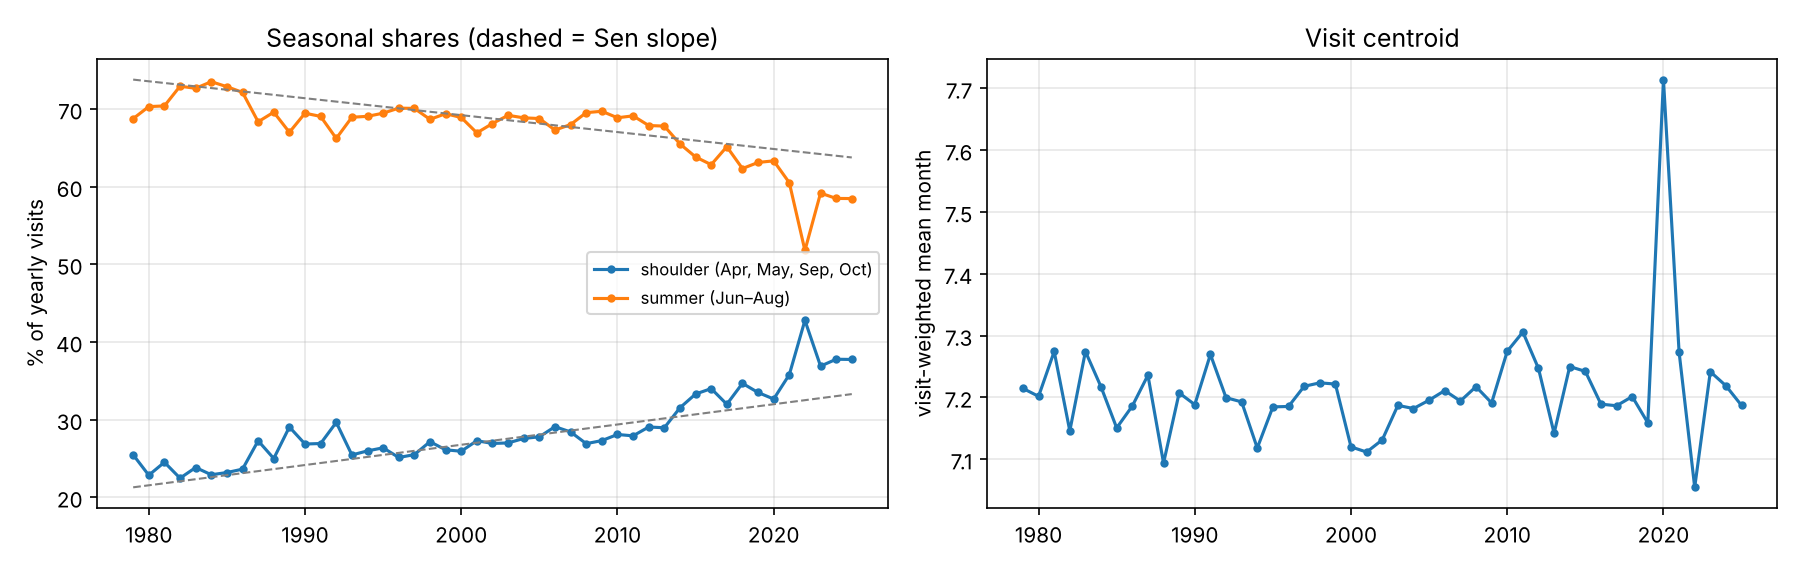
\includegraphics[width=0.9\textwidth]{q2_shoulder_share.png}
\caption{Seasonal shares of visits and the visit-weighted mean month, 1979--2025.}\label{fig:p3climate}
\end{figure}

\subsection{Shocks and forecasting}
Counterfactual SARIMA and ETS forecasts show that the 1988 fires, COVID and the 2022 flood were each over within 3--4 months. The flood was the costliest (1.1--2.5 million visits in its first year) and only COVID was followed by a rebound above normal. In rolling forecasts from 192 origins (2010--2019 targets), no model significantly beats ``same month last year'': the best single model, SARIMA with $d=0$ and drift, has MASE 1.18 at one month ahead against 1.28 for seasonal naive (Diebold--Mariano $p=0.48$), and forecast combinations are best by 3--4\% but not significantly. The $d=0$ model's 2026 forecast is within 6.8\% of the preliminary data so far.

\subsection{Answer to RQ3}
Wolves did not move park-wide visitor numbers. Policy, climate and a very regular season did. A wolf signal appears only in North-gate winter traffic, where it is suggestive but not conclusive.

%=====================================================================
\section{Part 4: Isle Royale wolves and moose}
%=====================================================================
\subsection{Why Isle Royale}
Isle Royale (544\,km$^2$, Lake Superior) has had wolves and moose and almost nothing else since 1949: no hunting, no bison or elk, and almost no migration. If wolves matter for their prey, the signal should be clearest here (Figure~\ref{fig:ir}). Part~4 wrote the shared model settings as a code module (\texttt{tsa\_spec.py}, version 1.3), which the synthesis also runs on Yellowstone.

\begin{figure}[H]
\centering
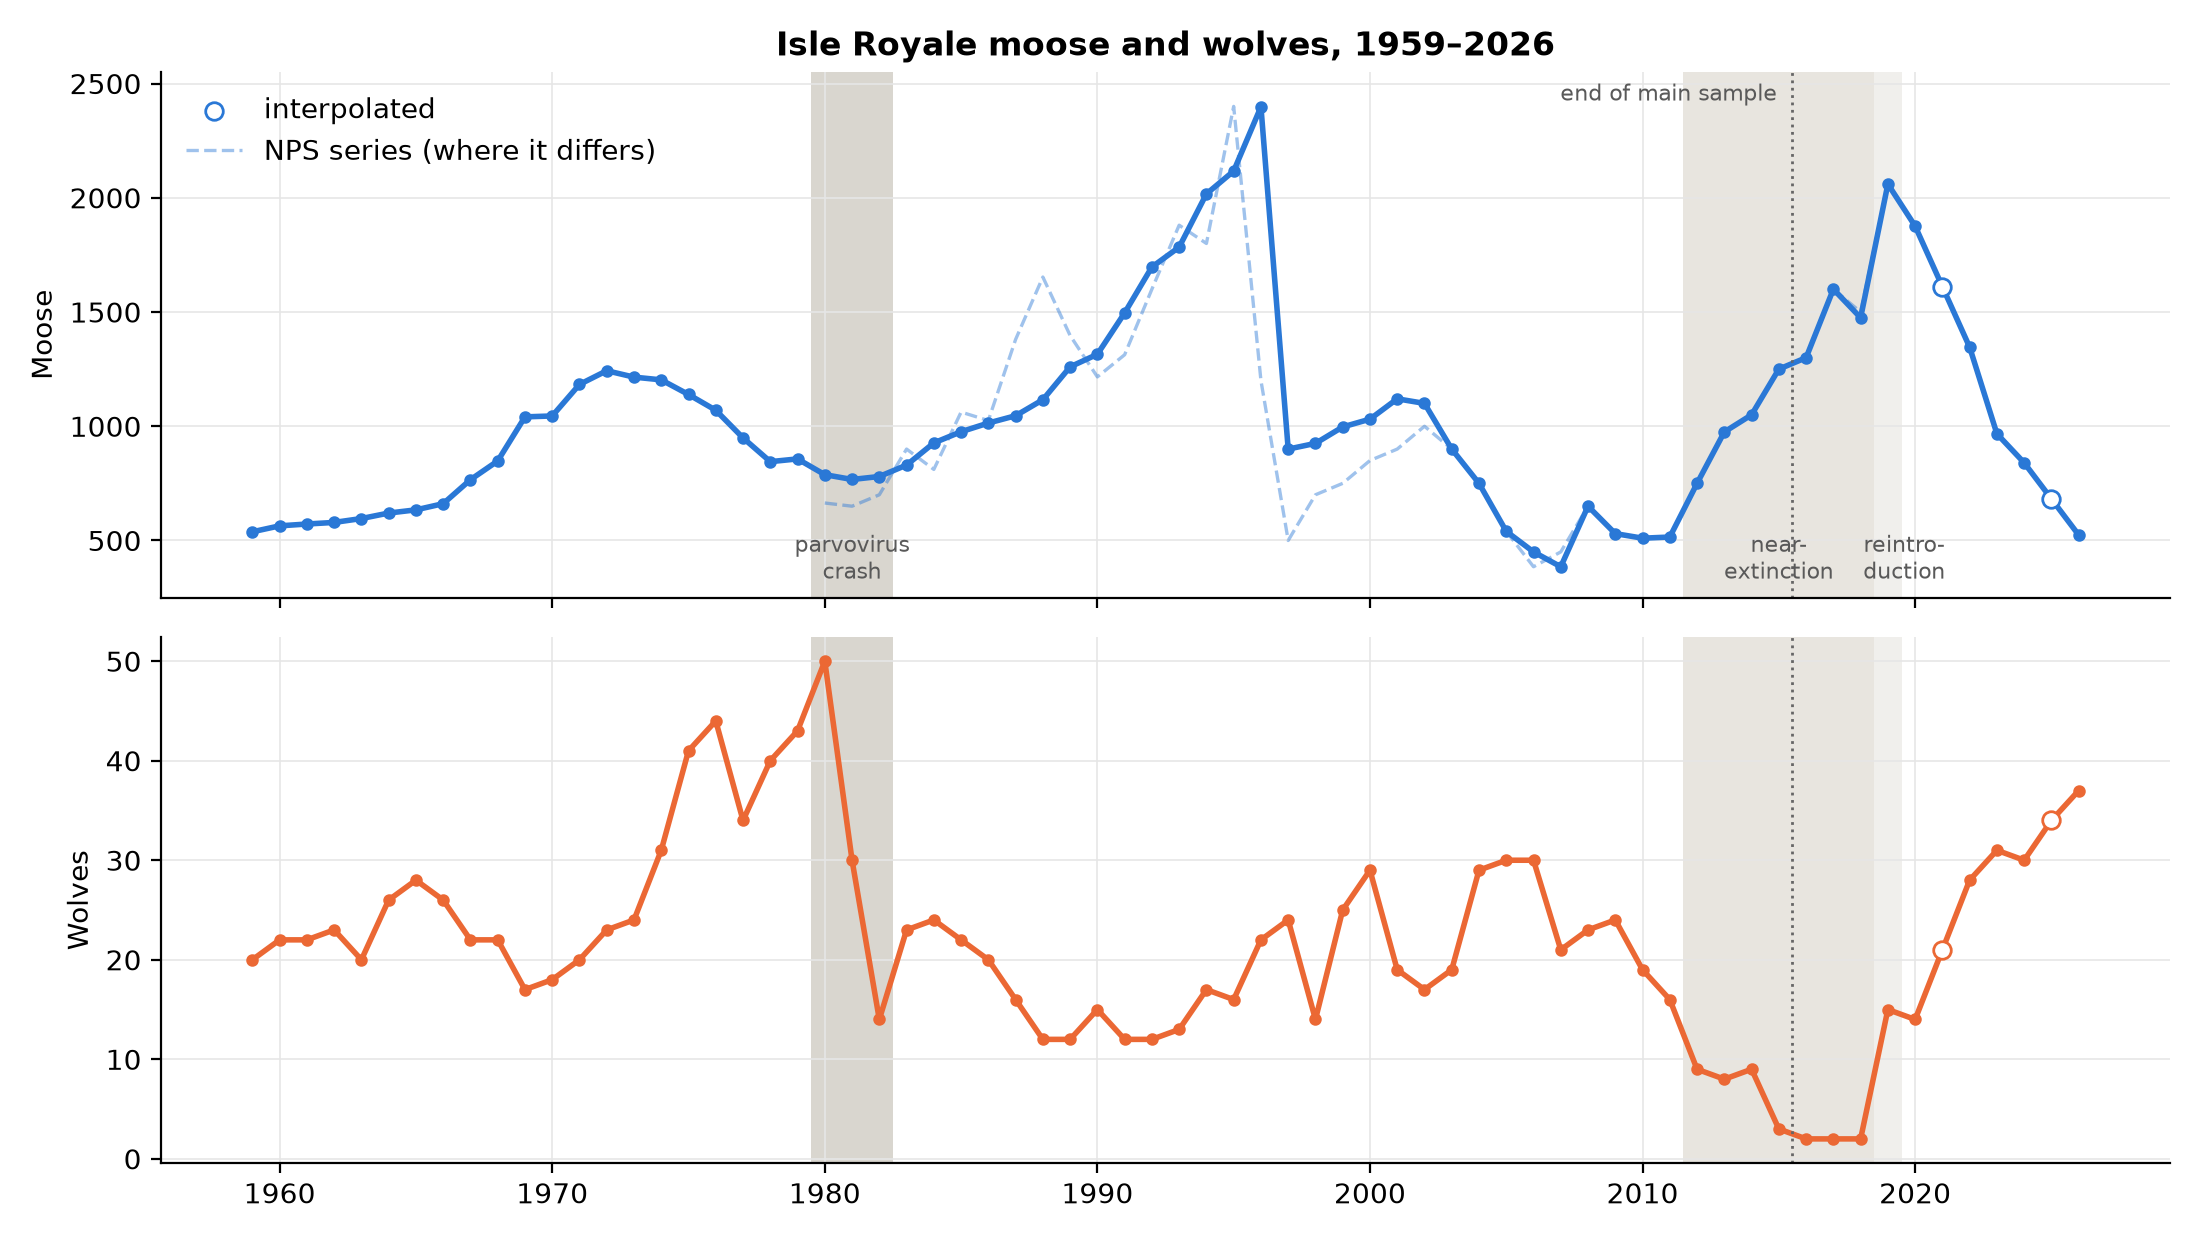
\includegraphics[width=0.85\textwidth]{IR_01_series.png}
\caption{Isle Royale moose (top) and wolves (bottom), 1959--2026. Shaded: parvovirus crash, near-extinction and reintroduction.}\label{fig:ir}
\end{figure}

\subsection{Time-series results}
Growth rates are stationary; log levels are inconclusive. Moose growth is white noise against its own past (every AR/MA term $p\ge0.67$), but this does not mean moose follow a random walk: wolves predict moose growth once they are in the model, density pulls the population back, and AR(1) on log moose gives $\phi=0.88$ (half-life about 6 years). The model, a linearised predator--prey equation, is
\begin{equation}
r_{M,t}=\mu+\beta_W\,\frac{W_{t-1}}{10}+\beta_D\log M_{t-1}+\varepsilon_t .
\end{equation}
\begin{itemize}
\item \textbf{ARIMAX.} With density, each additional ten wolves lowers moose growth by 8.0 percentage points (95\% CI $-16.0$ to $-0.1$; $p=0.047$), and doubling moose lowers growth by about 12 points. The combined model is best by AIC and BIC. The wolf effect is negative in all five robustness checks and significant in three. Residuals pass Ljung--Box ($p=0.96$) and ARCH ($p=0.96$). The coefficient implies about 8 moose killed per wolf per year at 1{,}000 moose, close to the observed field average of 8.4.
\item \textbf{Granger causality.} Wolves Granger-cause moose in every version: VAR(1) $p=0.011$; lags 1--4 $p=0.002$--$0.021$; without the 1997 crash $p=0.034$; Toda--Yamamoto levels test $p=0.006$--$0.017$. Moose do not Granger-cause wolves at one year ($p=0.18$), but moose 1--3 years back predict wolf growth ($p=0.026$), and wolf numbers track moose about 8 years later.
\item \textbf{Cointegration and forecasting.} Johansen rank 0: no fixed long-run ratio. Over 1990--2015, ARIMAX with wolves beats drift by 6.2\% in MAPE; no model foresaw the 1997 crash.
\item \textbf{Cycle.} The periodogram peaks at 28.5 years for both species, the second-lowest frequency resolvable in 57 years, so the cycle length is approximate.
\end{itemize}
For this report we also checked the VAR residuals: they pass the Portmanteau test at every lag used ($p=0.20$ for VAR(1), 0.47--0.71 for VAR(2)--VAR(4)), so the Granger results stand.

\begin{figure}[H]
\centering
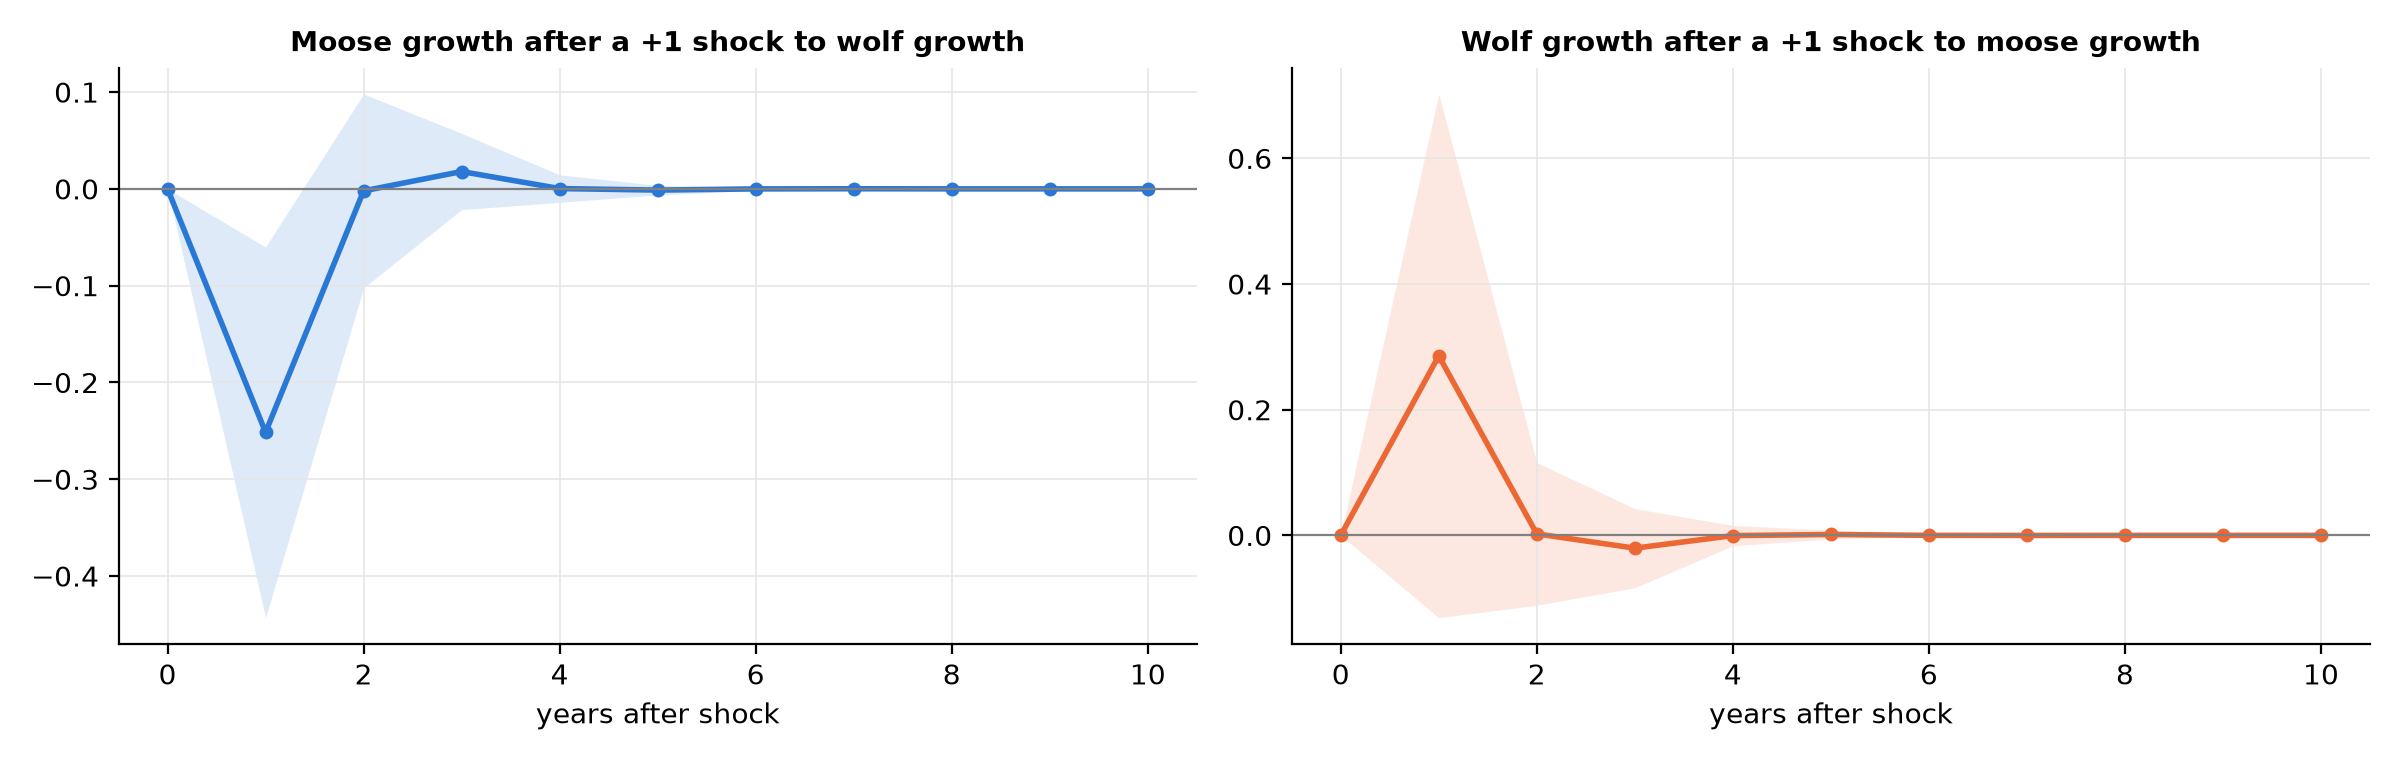
\includegraphics[width=0.9\textwidth]{IR_05_var_irf.png}
\caption{Impulse responses from the Isle Royale VAR(1), with 95\% bands.}\label{fig:irf}
\end{figure}

\subsection{Predator--prey equations and extinction risk}
In a discrete-time moose model, both predation forms beat logistic growth without wolves by 7--9 AIC points, but prey-dependent and ratio-dependent killing differ by only 1.4, so the counts cannot choose between them. The prey-dependent version gives realistic kill rates (8.0 moose per wolf per year) and a wolf balance point of 8.4, exactly the observed average. Whole-system ODE fits (Lotka--Volterra and Rosenzweig--MacArthur) follow the timing of the rises and falls but miss the extremes, and no fit with plausible parameters sustains a cycle.

Simulating the prey-dependent model 10{,}000 times from 1990 (1{,}315 moose, 15 wolves) with environmental and demographic noise, wolves fell to two or fewer by 2016 in 52\% of runs, and the observed 2016 count sits at the 42nd percentile (Figure~\ref{fig:ext}). Without demographic noise the risk is 3\%: the collapse was driven by small numbers.

\begin{figure}[H]
\centering
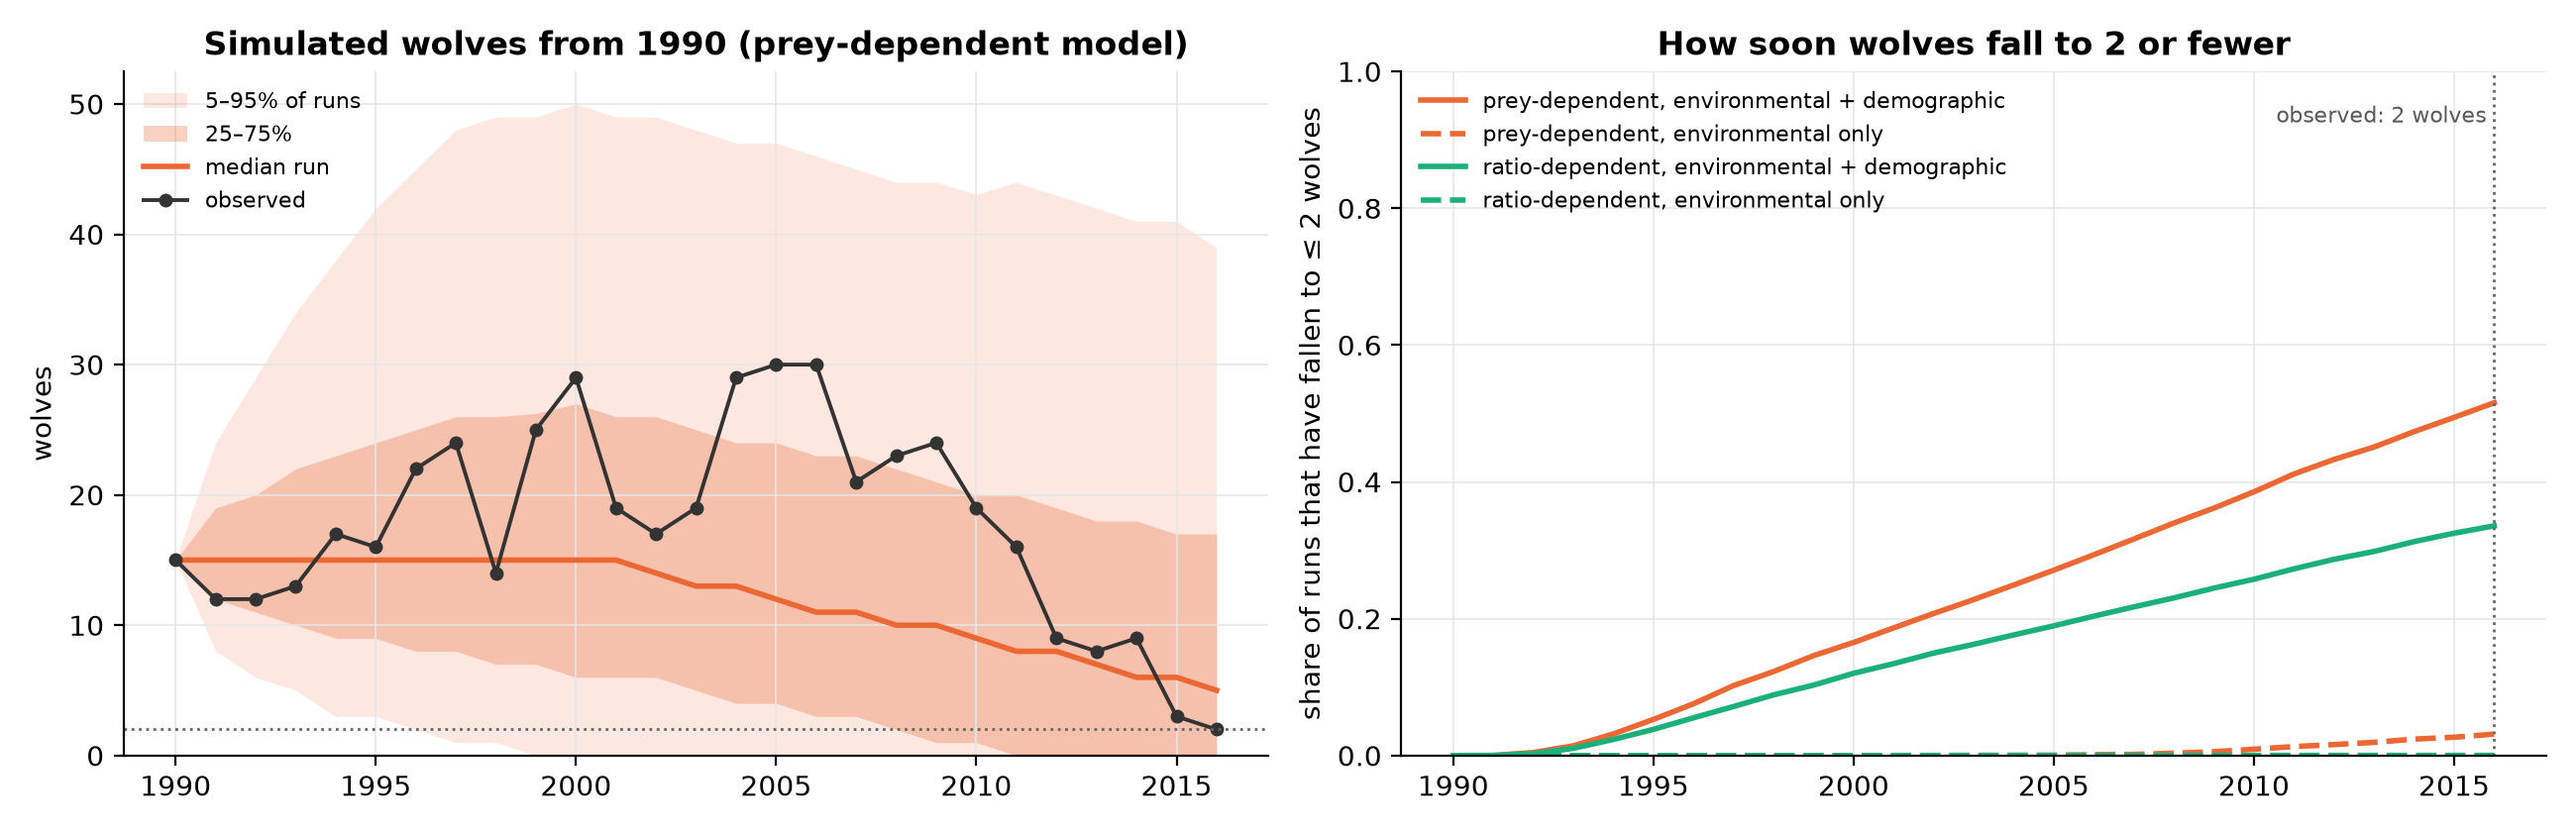
\includegraphics[width=\textwidth]{IR_11_extinction_curves.png}
\caption{Simulated wolf numbers from 1990 (left) and the share of runs at two or fewer wolves by each year (right).}\label{fig:ext}
\end{figure}

\subsection{Answer to RQ4}
On Isle Royale wolves measurably slow moose growth and wolves follow moose with a delay of about 8 years. The 2012--2016 wolf collapse was a likely outcome for a population this small and isolated.

%=====================================================================
\section{Synthesis}
%=====================================================================
\subsection{Same model, two parks}
To compare the systems fairly, both datasets were re-run with Part~4's unchanged specification: prey log growth on lagged wolf \emph{levels}, controlling for prey density, on the same 1984--2015 window and the same forecast years. This differs from Part~1's headline predictor (lagged \emph{changes} in wolves), so it supplements rather than replaces that analysis.

\begin{table}[H]
\centering\small
\caption{Shared specification on both systems. Wolf coefficient in log-growth percentage points per ten wolves.}\label{tab:compare}
\begin{threeparttable}
\begin{tabular}{@{}llcccc@{}}
\toprule
Sample & System & Wolf coefficient [95\% CI] & $p$ & Granger $p$ & MAPE gain \\
\midrule
Native windows & Yellowstone & $-1.60$ [$-3.91$, $+0.71$] & 0.175 & 0.142 & $-2.5\%$ \\
 & Isle Royale & $-8.04$ [$-15.96$, $-0.11$] & 0.047 & 0.011 & $+6.2\%$ \\
1984--2015 & Yellowstone & $-1.02$ [$-3.00$, $+0.96$] & 0.312 & 0.530 & $-5.3\%$ \\
 & Isle Royale & $-23.66$ [$-38.61$, $-8.71$] & 0.002 & 0.009 & $+8.2\%$\tnote{a} \\
\bottomrule
\end{tabular}
\begin{tablenotes}\footnotesize
\item[a] On the 22 forecast years shared with Yellowstone.
\end{tablenotes}
\end{threeparttable}
\end{table}

\begin{figure}[H]
\centering
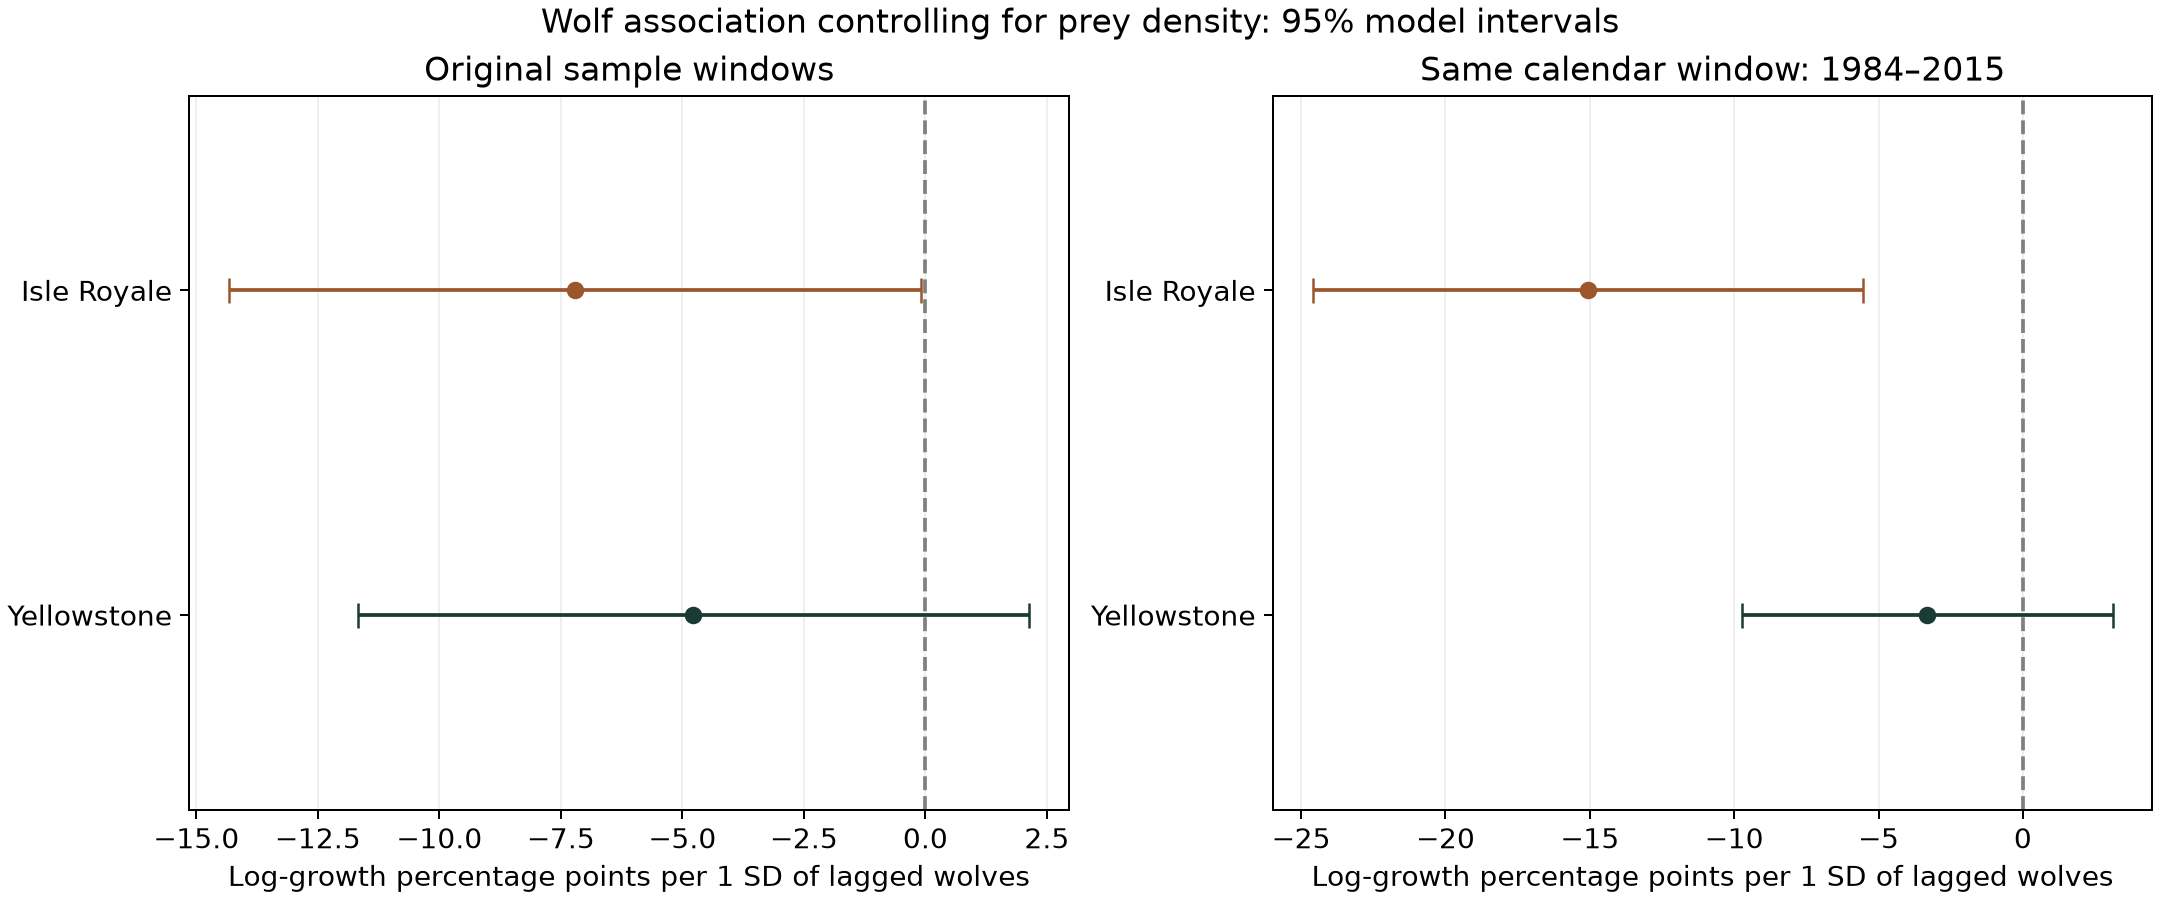
\includegraphics[width=0.92\textwidth]{wolf_effect_comparison.png}
\caption{Density-adjusted wolf association per standard deviation of lagged wolves, with 95\% model intervals.}\label{fig:compare}
\end{figure}

Under the same model, wolves carry clear predictive information about prey on Isle Royale and not in Yellowstone (Table~\ref{tab:compare}, Figure~\ref{fig:compare}). This does not prove that wolves have a weaker ecological effect in Yellowstone: the sample periods, survey methods, geography and wolf histories differ, and the difference between a significant and a non-significant $p$-value is not itself a test of a difference between systems. It is consistent with a wolf signal in Yellowstone being masked by hunting, bison, climate and changing survey methods.

\subsection{Granger causality and residual checks across the project}
\begin{table}[H]
\centering\small
\caption{Granger causality and white-noise checks, by part.}\label{tab:granger}
\begin{tabularx}{\textwidth}{@{}l Y Y@{}}
\toprule
Part & Granger causality & Residuals white noise? \\
\midrule
1 Elk and wolves & Wolves$\rightarrow$elk $p=0.18$; elk$\rightarrow$wolves $p=0.80$ (VAR(1), 1997--2025) & ARIMAX: yes (Ljung--Box $p\ge0.64$, ARCH $p\ge0.11$). VAR: yes (Portmanteau $p=0.54$) \\
2 Vegetation and water & No driver$\rightarrow$riverside greenness (all $p\ge0.20$); snow$\rightarrow$next year's river $p\ge0.19$; strong same-year link & Yes after fixes: SARIMA reselected, AR(1) errors for one stream, extra VAR lag for low flow; GARCH residuals white in practice \\
3 Visitation & Temperature$\rightarrow$visits $p=0.23$; strong same-month link & VAR(24): yes per series. SARIMA: yes at lags 12--36, heavy tails \\
4 Isle Royale & Wolves$\rightarrow$moose $p=0.011$ (lags 1--4: 0.002--0.021); moose$\rightarrow$wolves $p=0.18$ & ARIMAX: yes ($p\ge0.96$). VAR: yes (Portmanteau $p=0.20$) \\
\bottomrule
\end{tabularx}
\end{table}

Isle Royale is the only system in which wolves Granger-cause their prey (Table~\ref{tab:granger}). Elsewhere, the links that exist operate within the same period, not with a lag.

\subsection{The chain, link by link}
\begin{table}[H]
\centering\small
\caption{Strength of evidence for each link of the cascade.}\label{tab:chain}
\begin{tabularx}{\textwidth}{@{}l Y l@{}}
\toprule
Link & Evidence & Strength \\
\midrule
Wolves $\rightarrow$ prey numbers & Clear on Isle Royale ($p=0.002$--$0.047$; Granger $p=0.011$); uncertain in Yellowstone ($p=0.12$--$0.41$) & Mixed \\
Elk $\rightarrow$ streamside vegetation & Same-year browning with more elk ($p=0.006$); greening only on Blacktail Creek; no lagged effect & Partial \\
Snow and water $\rightarrow$ river & Melt-out sets river timing ($R^2=0.78$); pulse 13 days earlier since 1950; summer low flow falling & Strong \\
Floods $\rightarrow$ braided channels & 1996--97 and 2022 floods cut riverside greenness by up to 6 SD; confounded with 1995 & Strong \\
Wolves $\rightarrow$ visitors & No park-wide winter rise (rules out $>+1.5\%$); North-gate cars track wolves (elasticity $\approx0.3$) & Weak \\
\bottomrule
\end{tabularx}
\end{table}

%=====================================================================
\section{Limitations}
%=====================================================================
\begin{itemize}
\item \textbf{Short series.} Most models use 25--56 annual values, so tests have low power to detect moderate effects.
\item \textbf{Changing data definitions.} Imputed and re-surveyed elk counts, the 1993 visitor counting change, Landsat sensor changes and the reconstructed Isle Royale moose series all affect comparability. Each is flagged and tested with sensitivity runs, but cannot be fully removed.
\item \textbf{Coincident events.} The wolf release (1995--96), the record floods (1996--97), the 1988 fires, heavy hunting in the late 1990s and counting changes sit within a few years of each other.
\item \textbf{Spatial mismatch.} Wolf counts cover northern-range packs while whole-herd elk counts include migrants outside the park; the river gauge integrates a large basin; 30\,m pixels mix willows with gravel and water.
\item \textbf{Prediction is not causation.} Granger tests and ARIMAX show predictive information only. Establishing the vegetation mechanism needs browsing, plant height and water-table data.
\item \textbf{Model assumptions.} Several residual series are heavy-tailed, so some $p$-values and prediction intervals are approximate; the flood return period depends on the assumed tail.
\end{itemize}

%=====================================================================
\section{Conclusion}
%=====================================================================
Wolves matter most clearly where the system is simple. On Isle Royale, the same models that find little in Yellowstone show wolves predicting and limiting moose, with wolves following moose about eight years later. In Yellowstone, wolf changes carry only an uncertain signal for elk growth. Streamside recovery appears on the small willow-lined creek where the cascade was first reported, and elk increases go with a browner riverside in the same summer, but on the large braided rivers floods, snow and water dominate. Snowmelt and the river now peak about two weeks earlier than in 1950 and summer low flow is falling, and visitors follow climate and policy rather than wolves. A trophic cascade is consistent with parts of this evidence, but it cannot be established from annual time series alone.

\newpage
%=====================================================================
\begin{thebibliography}{10}\small
\bibitem[Box et~al.(2015)]{box2015} Box, G. E. P., Jenkins, G. M., Reinsel, G. C., \& Ljung, G. M. (2015). \emph{Time Series Analysis: Forecasting and Control} (5th ed.). Wiley.
\bibitem[Eberhardt et~al.(2007)]{eberhardt2007} Eberhardt, L. L., White, P. J., Garrott, R. A., \& Houston, D. B. (2007). A seventy-year history of trends in Yellowstone's northern elk herd. \emph{Journal of Wildlife Management}, 71, 594--602.
\bibitem[Engle(1982)]{engle1982} Engle, R. F. (1982). Autoregressive conditional heteroscedasticity with estimates of the variance of United Kingdom inflation. \emph{Econometrica}, 50(4), 987--1007.
\bibitem[Granger(1969)]{granger1969} Granger, C. W. J. (1969). Investigating causal relations by econometric models and cross-spectral methods. \emph{Econometrica}, 37(3), 424--438.
\bibitem[Hobbs et~al.(2024)]{hobbs2024} Hobbs, N. T., Johnston, D. B., Marshall, K. N., Wolf, E. C., \& Cooper, D. J. (2024). Does restoring apex predators to food webs restore ecosystems? Large carnivores in Yellowstone as a model system. \emph{Ecological Monographs}, 94, e1598.
\bibitem[Hock(2003)]{hock2003} Hock, R. (2003). Temperature index melt modelling in mountain areas. \emph{Journal of Hydrology}, 282, 104--115.
\bibitem[Ljung and Box(1978)]{ljungbox1978} Ljung, G. M., \& Box, G. E. P. (1978). On a measure of lack of fit in time series models. \emph{Biometrika}, 65(2), 297--303.
\bibitem[MacNulty et~al.(2016)]{macnulty2016} MacNulty, D. R., Stahler, D. R., Wyman, C. T., Ruprecht, J., \& Smith, D. W. (2016). The challenge of understanding northern Yellowstone elk dynamics after wolf reintroduction. \emph{Yellowstone Science}, 24(1).
\bibitem[Marshall et~al.(2013)]{marshall2013} Marshall, K. N., Hobbs, N. T., \& Cooper, D. J. (2013). Stream hydrology limits recovery of riparian ecosystems after wolf reintroduction. \emph{Proceedings of the Royal Society B}, 280, 20122977.
\bibitem[Ripple and Beschta(2012)]{ripple2012} Ripple, W. J., \& Beschta, R. L. (2012). Trophic cascades in Yellowstone: The first 15 years after wolf reintroduction. \emph{Biological Conservation}, 145(1), 205--213.
\end{thebibliography}

\appendix
\section{Reproducibility}
All code and data are in the project repository, one folder per part. Notebooks are numbered uniquely across the project and run in order within each folder.
\begin{table}[H]
\centering\small
\begin{tabularx}{\textwidth}{@{}l l Y@{}}
\toprule
Folder & Notebooks & Contents \\
\midrule
\texttt{01\_yellowstone\_elk\_wolves} & 01--05 & Data audit, drivers, VAR and Granger, forecasts, breaks, removals, viability, state space; \texttt{scripts/run\_all.py} rebuilds everything \\
\texttt{02\_vegetation\_snow\_river} & 12, then 11 & Snow and river (12), riverside vegetation (11), including Granger and residual checks \\
\texttt{03\_park\_visitation} & 13--14 & Base SARIMA and forecasting (13); interventions, climate, shocks, North gate (14) \\
\texttt{04\_isle\_royale} & 08--10 & Time-series analysis (08), predator--prey ODEs (09), stochastic simulation (10); shared settings in \texttt{scripts/tsa\_spec.py} \\
\texttt{05\_synthesis} & -- & \texttt{scripts/build\_comparison.py} re-runs both systems with the shared settings \\
\bottomrule
\end{tabularx}
\end{table}

\end{document}
